%%\documentclass[twocolumn,pdflatex,sn-basic,NameDate]{sn-jnl}% Basic, two column unnumbered refs
\documentclass[twocolumn,pdflatex,sn-nature]{sn-jnl}% Basic, one column numbered refs
%%\documentclass[pdflatex,sn-nature]{sn-jnl}% Basic, one column unnumbered refs

%%%% Standard Packages

\usepackage{graphicx}%
\usepackage{multirow}%
\usepackage{amsmath,amssymb,amsfonts}%
\usepackage{amsthm}%
\usepackage{mathrsfs}%
\usepackage[title]{appendix}%
\usepackage{xcolor}%
\usepackage{textcomp}%
\usepackage{manyfoot}%
\usepackage{booktabs}%
\usepackage{algorithm}%
\usepackage{algorithmicx}%
\usepackage{algpseudocode}%
\usepackage{listings}%


\usepackage{anyfontsize}%
\usepackage[separate-uncertainty=true,multi-part-units=single]{siunitx}%
\usepackage{tabularx}

\pdfstringdefDisableCommands{%
  \def\\{}%
  \def\textsuperscript#1{<#1>}%
}

%%%%

% \raggedbottom
\unnumbered% uncomment this for unnumbered level heads

% Zach's commands

% Units
\DeclareSIUnit\molar{\textsc{m}}
\DeclareSIUnit\mM{\milli\molar}
\DeclareSIUnit\uM{\micro\molar}
\DeclareSIUnit\nM{\nano\molar}
\DeclareSIUnit\angstrom{\text {Å}}

% Taxonomy
\newcommand\ec{\textit{E.~coli}}
\newcommand\ecfull{\textit{Escherichia coli}}
% \newcommand\mtb{\textit{M.~tuberculosis}}
\newcommand\mtb{Mtb}
\newcommand\mtbfull{\textit{Mycobacterium tuberculosis}}
\newcommand\msmegfull{\textit{Mycolicibacterium smegmatis}}
\newcommand\msmeg{\textit{M. smegmatis}}
\newcommand\pafull{\textit{Pseudomonas aeruginosa}}
\newcommand\pa{\textit{P. aeruginosa}}

% Protein variant and region designations
\newcommand\ftsbTM{FtsB\textsuperscript{TM}}
\newcommand\ftsbLQ{FtsB\textsuperscript{LQ}}
\newcommand\ftsbH{FtsB\textsuperscript{H}}
\newcommand\ftsbdLQ{FtsB\textsuperscript{$\Delta{}$LQ}}
\newcommand\ftsbdH{FtsB\textsuperscript{$\Delta{}$H}}
\newcommand\ftsbdLQdH{FtsB\textsuperscript{$\Delta{}$LQ$\Delta{}$H}}
\newcommand\ftsbdCdH{FtsB\textsuperscript{$\Delta{}$C$\Delta{}$H}}
\newcommand\ftsbdC{FtsB\textsuperscript{$\Delta{}$C}}
\newcommand\permN{PerM\textsuperscript{n1}}

\begin{document}

\title[Article Title]{\mtbfull{} FtsB and PerM interact via a C-terminal helix in FtsB to modulate cell division}

\author[1]{\fnm{João Ramalheira} \sur{Ferreira}}
\equalcont{These authors contributed equally to this work.}

\author[1]{\fnm{Ruilan} \sur{Xu}}
\equalcont{These authors contributed equally to this work.}

\author*[1]{\fnm{Zach} \sur{Hensel}}\email{zach.hensel@itqb.unl.pt}

\affil[1]{\orgdiv{ITQB NOVA}, \orgname{Universidade NOVA de Lisboa}, \orgaddress{\street{Av. da República}, \city{Oeiras}, \postcode{2780-157}, \country{Portugal}}}

\abstract{Latent infection by \mtbfull{} (\mtb{}) impedes effective tuberculosis therapy and eradication. The protein PerM is essential for chronic \mtb{} infections in mice and acts via the divisome protein FtsB to modulate cell division. Using transgenic co-expression in \ecfull{}, we studied the \mtb{} PerM-FtsB interaction in isolation from other \mtb{} proteins, engineering PerM to enhance expression in the \ec{} membrane. We confirmed the reported instability of \mtb{} FtsB, and we linked FtsB instability to a segment of FtsB predicted to bind cell-division proteins FtsL and FtsQ. Though narrowly conserved, the PerM-FtsB interaction emerges as a potential target as part of therapy targeting persistent infections by disrupting regulation of cell division. Using fluorescence microscopy, we found that stability of both FtsB and PerM hinges on their interaction via a C-terminal helix in FtsB. Molecular dynamics results supported the observation that FtsB stabilized PerM, and suggested that interactions at the PerM-FtsB interface differ from our initial structure prediction in a way that is consistent with PerM sequence conservation. Integrating protein structure prediction, molecular dynamics and single-molecule microscopy, our approach is primed to screen potential inhibitors of the PerM-FtsB interaction and can be straightforwardly adapted to explore other putative interactions.}

\keywords{\mtbfull{}, cell division, single-molecule microscopy, molecular dynamics}

\maketitle

\section{Introduction}\label{sec1}

\mtbfull{} (\mtb{}) is a major contributor to preventable deaths by infectious disease and has infected approximately a quarter of the global population \citep{houbenGlobalBurdenLatent2016}. Most infections progress to latent tuberculosis infection (LTBI), characterized by an immunological response to \mtb{} antigens without clinical signs of active TB \citep{whoLatentTuberculosisInfection2018}. Preventing establishment and reactivation of LTBI is a growing priority for TB elimination strategies, although uncertainties continue to limit measurements of the relative burdens of new TB infections and LTBI reactivation \citep{daleQuantifyingRatesLate2021}. Protocols that reduce the duration and adverse effects of treatment can reduce LTBI burden by improving upon completion rates for preventative treatment \citep{assefaEfficacySafetyDifferent2023}. Furthermore, imperfect treatment over long periods can contribute to acquisition of drug resistance \citep{liAcquiredResistanceIsoniazid2021}. Consequently, it is imperative to better understand how \mtb{} infections persist to establish LTBI in order to inform strategies for novel LTBI treatments with higher efficacy, shorter durations, and reduced risk of drug resistance.

A potential strategy to prevent establishment and reactivation of LTBI is to characterize and target mechanisms through which \mtb{} persists through host-induced stress \citep{dartoisAntituberculosisTreatmentStrategies2022}. The actinomycete protein PerM was one of 21 genes identified in a screen of transposon \mtb{} mutants with attenuated growth at pH~$4.5$ in media containing Tween 80, with most of the identified genes being associated with cell wall synthesis \citep{vandalMembraneProteinPreserves2008}. A subsequent study focused on PerM, finding that \mtb{} PerM knockout reduced growth during chronic mouse infection and increased $\beta$-lactam antibiotic susceptibility. Localization of fluorescently tagged PerM to dividing septa suggested a connection to cell division \citep{goodsmithDisruptionTuberculosisMembrane2015}. Further work demonstrated that PerM associates with the \mtb{} divisome, a protein complex orchestrating cell wall remodeling during division, and that PerM depletion can be complemented by overexpression of the divisome component FtsB \citep{wangPersistentMycobacteriumTuberculosis2019}. PerM was also recently identified by transposon sequencing to play an even more significant role in infecting mice in a background with weakened adaptive immune response \citep{meadeGenomewideScreenIdentifies2023}.

Recently, a covalent inhibitor of divisome formation based upon the structure of FtsB-FtsQ was developed and found to be active against drug-resistant \ec{} in an animal infection model \citep{paulussenCovalentProteomimeticInhibitor2022}. The \mtb{} proteome includes homologs of the five core \ec{} divisome proteins FtsQ, FtsL, FtsB, FtsW, and FtsI \citep{wuCharacterizationConservedNovel2018}, suggesting that a similar approach can target protein-protein interactions in the \mtb{} divisome. However, it is unknown whether PerM directly interacts with FtsB  \citep{wangPersistentMycobacteriumTuberculosis2019} and, if it does, whether there is a regulatory mechanism for PerM beyond impacting FtsB stability. PerM lacks known orthologs outside of actinomycetes \citep{goodsmithDisruptionTuberculosisMembrane2015}, so PerM interactions could potentially be targeted by specific therapies. However, no experimental structural data have been published on the PerM-FtsB interaction or on PerM alone to guide experimental design. Expression and purification of \mtb{} PerM and FtsB for structural study is likely to pose difficulties given that FtsB stability depends upon PerM co-expression in \mtb{} and \msmegfull{} \citep{wangPersistentMycobacteriumTuberculosis2019}. Furthermore, proteins such as PerM with a high number of transmembrane helices pose challenges for recombinant expression \citep{graveHighthroughputStrategyIdentification2022, korepanovaCloningExpressionMultiple2005}.

Recent insights into the molecular structure and regulatory mechanisms of the gram-negative divisome have been enabled by the confluence of protein structure prediction, cryogenic electron microscopy (Cryo-EM), and molecular dynamics (MD) simulations. The extension from prediction of monomers to protein complexes \citep{baekAccuratePredictionProtein2021, evansProteinComplexPrediction2022} facilitated rapid structure prediction of the core \ec{} divisome \citep{attaibiUpdatedModelDivisome2022, cravenModelInteractionsFtsQLB2022}. Analysis of a Cryo-EM structure of the \pafull{} divisome was largely consistent with predicted protein-protein interfaces, but also revealed a global conformational change absent in structure predictions \citep{kashammerCryoEMStructureBacterial2023}. All-atom MD simulations identified a similar conformational change within \qty{1}{us}, and further predicted interactions between the core divisome and \ec{} FtsN \citep{brittonConformationalChangesEssential2023}. However, limitations of this MD approach, such as uncertainty in structure predictions and limited MD timescales, call for experimental validation. Importantly, in silico predictions for FtsN were corroborated by experimental results in living cells \citep{parkEssentialDomainFtsN2023}.

In this work, we employed a combination of structure prediction, MD, and fluorescence microscopy to probe the predicted interaction between \mtb{} PerM and FtsB proteins. In our approach, \mtb{} PerM and FtsB were expressed \ec{} in order to directly attribute observations to changes in the \mtb{} proteins. First, we investigated conservation and dynamics at the predicted PerM-FtsB interface, identifying roles for conserved residues that are absent in structure predictions. Second, we showed that FtsB instability (when expressed in \ec{}) depends on a region predicted to bind FtsL and FtsQ, and that PerM expression in \ec{} can be enhanced by strategically modifying its N-terminal signal sequence. This enabled the quantification of the PerM-FtsB interaction via fluorescence correlation and single-molecule tracking. We found PerM expression in the \ec{} membrane to depend on the FtsB sequence predicted to mediate PerM-FtsB interaction. Lastly, we investigated MD simulations of \mtb{} divisome complexes suggestive of PerM regulatory complexity beyond FtsB stabilization.

\section{Results}

\subsection{Structure prediction and molecular dynamics of PerM-FtsB interaction}

In preliminary structure predictions, we identified a high-confidence predicted interaction between \mtb{} PerM and FtsB ($pDockQ \approx 0.6$ \citep{bryantImprovedPredictionProteinprotein2022}).
The predicted structure of PerM was largely consistent with previous predicted topology \citep{goodsmithDisruptionTuberculosisMembrane2015} except that two regions with hydrophobic residues in predicted transmembrane helices did not span the membrane in structure predictions (Fig.~\ref{fig1_1}A).
The topology remains N-in, C-in, with the predicted PerM structure consisting of two halves, each with the same topology (three transmembrane helices with a buried extracellular loop between the first two).
Preliminary molecular dynamics (MD) simulations showed that the predicted PerM-FtsB interaction persisted on the microsecond timescale.
To test stability of the structure of the predicted complex further, we carried out a three-stage MD protocol with \qty{100}{\ns} of equilibrium MD followed by \qty{500}{\ns} of accelerated molecular dynamics (aMD), and a final \qty{500}{\ns} of equilibrium MD.
Terminal residues lacking high local prediction confidence ($pLDDT < 50$) were omitted in constructing the simulation system of FtsB\textsuperscript{61--204} and PerM\textsuperscript{11--390}.
Fig.~\ref{fig1_1}A shows how the predicted extended structure of FtsB collapsed in the absence of interactions with other divisome components \citep{brittonConformationalChangesEssential2023,cravenModelInteractionsFtsQLB2022,attaibiUpdatedModelDivisome2022,kashammerCryoEMStructureBacterial2023}.
Interaction between transmembrane helices of PerM and FtsB was not predicted with high confidence and also did not exhibit persistent, specific interactions in MD.
Conversely, the predicted interaction between FtsB and a specific pocket in the periplasmic face of PerM was maintained throughout the aMD protocol and in a simulation replicate.

\begin{figure*}[htb]
\centering
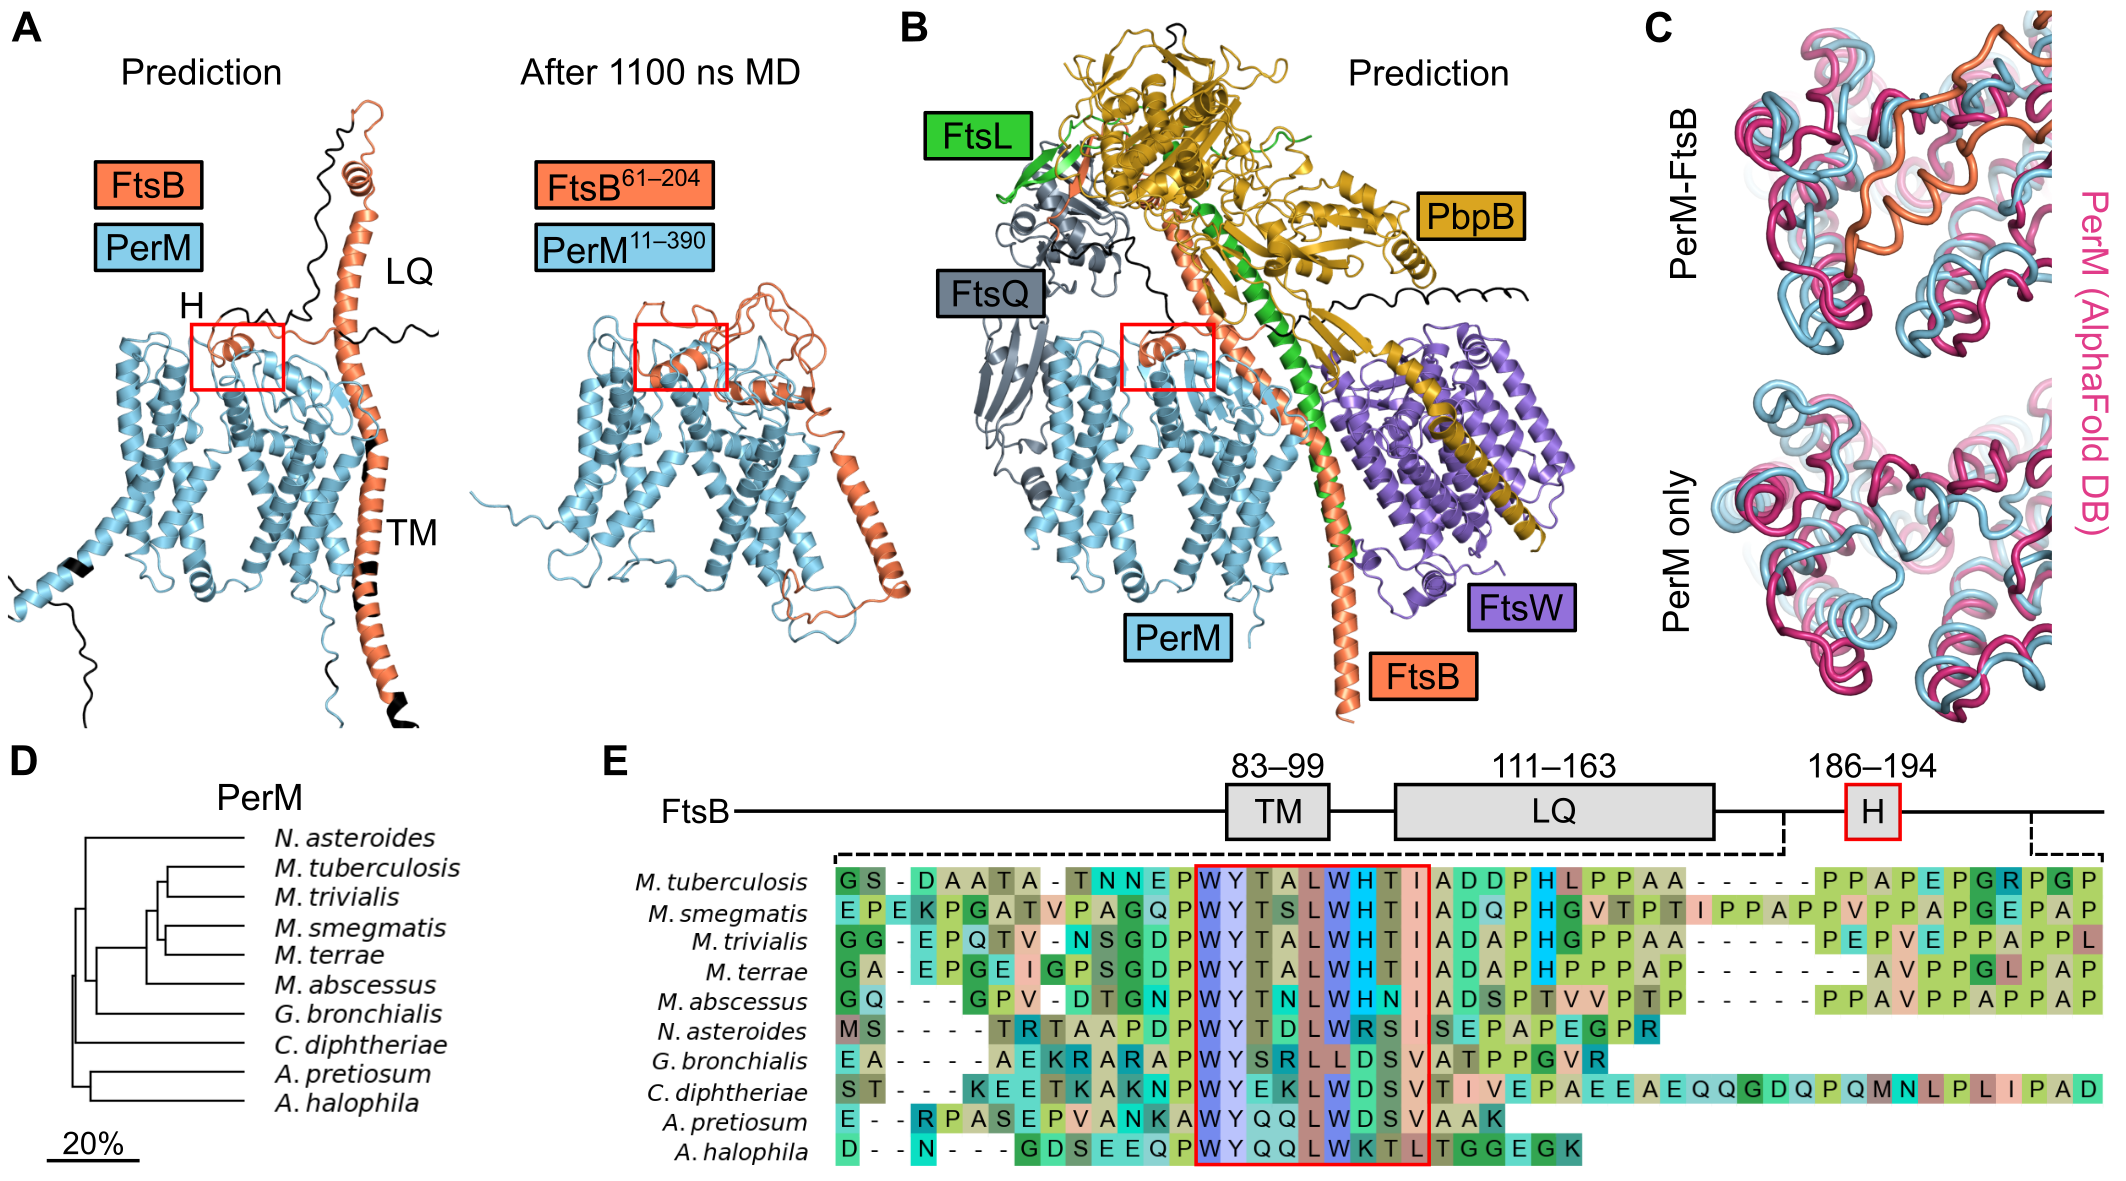
\includegraphics[width=1.0\textwidth]{../figures/fig1_1.png}
\caption{
    \textbf{A conserved, predicted \mtb{} PerM-FtsB interaction stabilizes PerM in MD.}
    (\textbf{A})~Left: predicted PerM-FtsB complex in which an $\alpha$~helix, \ftsbH{}, interacts with the periplasmic face of PerM. Transmembrane helix \ftsbTM{} and the region interacting with FtsL and FtsQ, \ftsbLQ{}, are indicated. Residues with $pLDDT < 50$ colored black. Right: final conformer following \qty{1.1}{\us} MD; PerM-\ftsbH{} interact persists, \ftsbLQ{} collapses, and \ftsbTM{} moves away from PerM.
    (\textbf{B})~Prediction for the \mtb{} divisome with inclusion of PerM. Terminal regions with $pLDDT < 50$ are omitted except for the FtsB C-terminus. All complexes in \textbf{A} and \textbf{B} are aligned by PerM C$\alpha$ atoms; the red box is placed at the same position relative to PerM for comparison of \ftsbH{} movement.
    (\textbf{C})~Final MD conformers for PerM-FtsB and for PerM alone are aligned by PerM C$\alpha$ atoms and compared to a PerM prediction  (AlphaFold DB P9WKN3-F1-model{\_}v4).
    (\textbf{D})~Phylogenetic tree for actinomycete species with predicted PerM-FtsB interactions. Branch length scaled by divergence in amino acid identity in pairwise sequence alignments of PerM.
    (\textbf{E})~Top: Diagram of \mtb{} FtsB defining the \ftsbTM{}, \ftsbLQ{}, and \ftsbH{} regions. Bottom: Multiple sequence alignment of a region near the C-terminus of FtsB for actinomycete species illustrates conservation of residues in \ftsbH{} and diversity in FtsB C-termini.
}\label{fig1_1}
\end{figure*}

We also found that a prediction of the core \mtb{} divisome with the addition of PerM was consistent with PerM interacting with the core divisome without obviously disrupting interactions between core divisome components (Fig. \ref{fig1_1}B).
Within this complex, PerM was only predicted to interact with FtsB.
Based on these predictions, we identified three regions of interest in \mtb{} FtsB: the predicted transmembrane helix, \ftsbTM{} (FtsB 83--99), the region predicted to interact with FtsL and FtsQ, \ftsbLQ{} (FtsB 111--163), and a span of hydrophobic residues forming an $\alpha$~helix predicted to interact with PerM, \ftsbH{} (FtsB 186--194).
Although C-terminal residues following \ftsbH{} were predicted to thread between the PbpB anchor and head domains, there were no high-confidence predictions for this region.

In order to see the impact of FtsB on PerM, we replicated the three-stage MD protocol using PerM alone.
Final conformers for PerM-FtsB and PerM simulations are shown in Fig.~\ref{fig1_1}C and compared to a recent PerM structure prediction from the AlphaFold Protein Structure Database \citep{varadiAlphaFoldProteinStructure2022}.
Surprisingly, we found that the final conformer in the monomeric PerM simulation differed from the predicted PerM structure ($RMSD=\qty{3.47}{\angstrom}$) to a greater extent than final conformers in PerM-FtsB simulation replicates (\qty{2.50}{\angstrom} and \qty{2.21}{\angstrom}).
The largest structural changes were seen in the predicted \ftsbH{} binding pocket.

Since our structure predictions were informed by information encoded in multiple sequence alignments, we searched for and identified PerM orthologs in actinomycete species (Fig.~\ref{fig1_1}D).
For each, we also identified the corresponding FtsB sequence and predicted the structures of PerM-FtsB complexes.
In every species tested there was a predicted interaction between PerM and \ftsbH{} with the same orientation of \ftsbH{} on the periplasmic face of PerM (Supplementary Fig.~\ref{figS1}).
Further, there is little difference in the lengths of regions linking \ftsbLQ{} and \ftsbH{}.
PerM-FtsB complexes differed, however, in the predicted position of \ftsbTM{} relative to PerM.
We constructed a multiple sequence alignment of FtsB to investigate the basis for conserved, predicted PerM-FtsB interaction and found that \ftsbH{} was highly conserved (Fig.~\ref{fig1_1}E) with near perfect conservation of hydrophobic residues predicted to interact with PerM (W\textsuperscript{186}, Y\textsuperscript{187}, L\textsuperscript{190}, and W\textsuperscript{191}).

Next, we investigated the structural basis for specific PerM-FtsB interaction. Fig.~\ref{fig1_2} illustrates the evolution of the FtsB binding pocket in PerM during MD.
In both simulation replicates, we observed that a large, hydrophobic binding pocket tightened around \ftsbH{}, and around FtsB W\textsuperscript{186} in particular. 
Residues in the W\textsuperscript{186} binding pocket include PerM G\textsuperscript{228}, which was perfectly conserved in PerM sequences in species that we analyzed.
Remarkably, specific hydrogen bonds between PerM and conserved FtsW residues emerged, none of which were present in structure predictions.
Fig.~\ref{fig1_1}B shows that evolution of the PerM-FtsB binding interface was reproducible.

\begin{figure*}[htb]
    \centering
    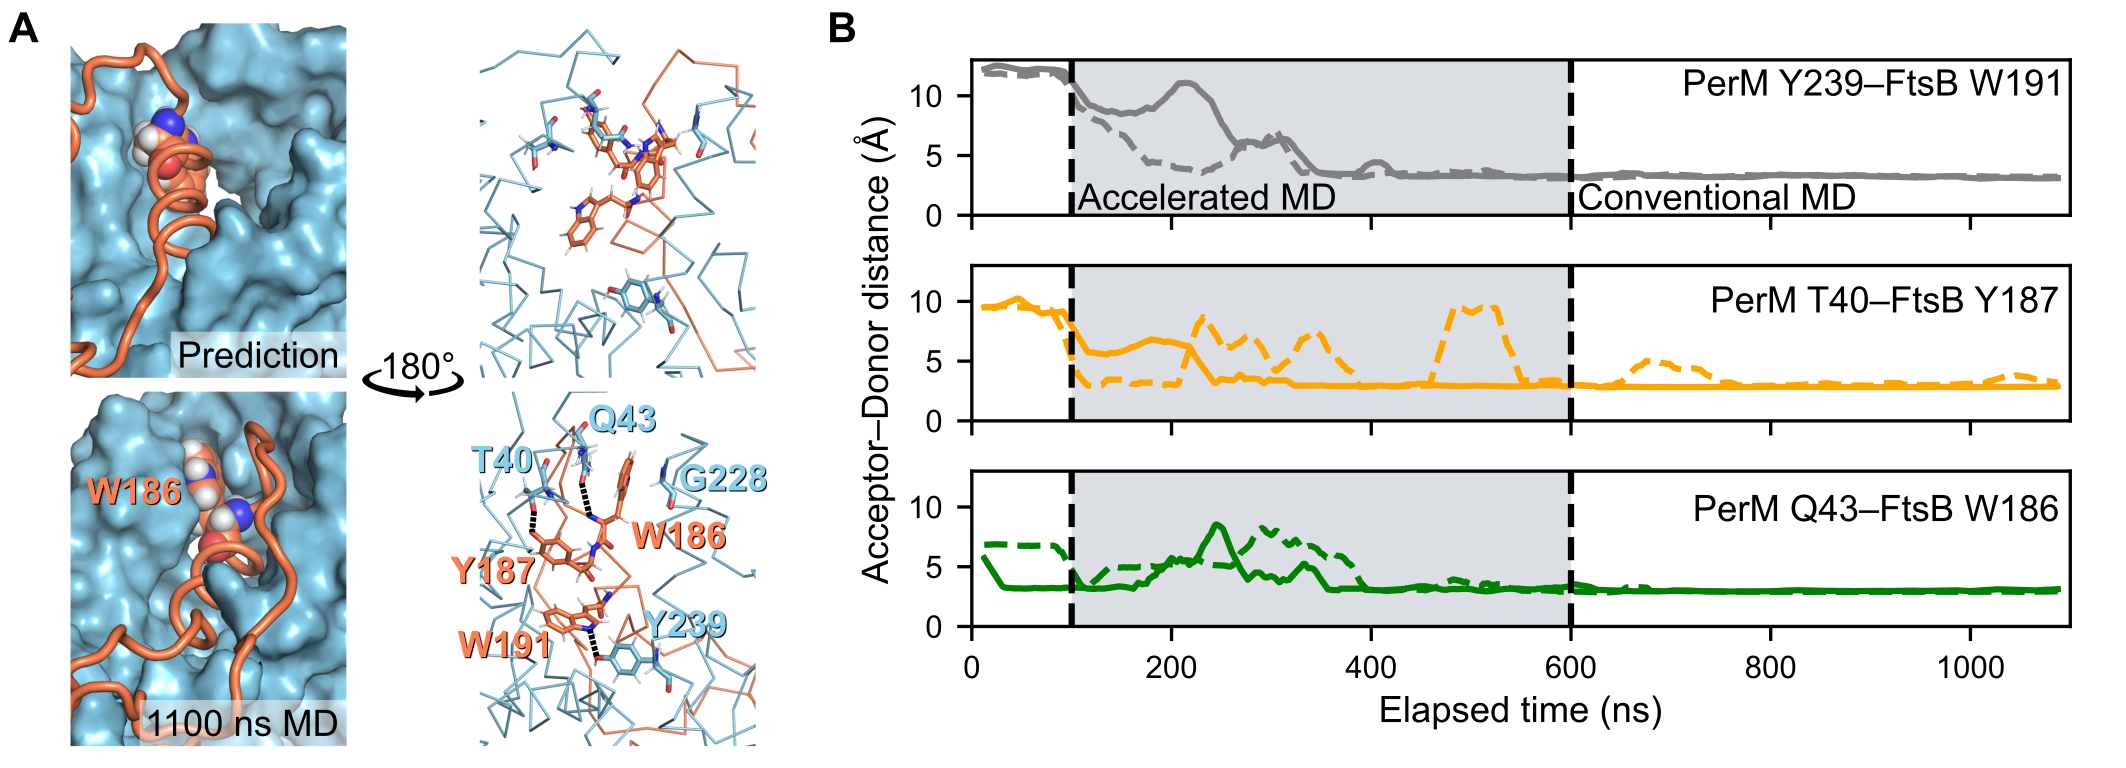
\includegraphics[width=1.0\textwidth]{../figures/fig1_2.png}
    \caption{
        \textbf{Reproducible dynamics at the PerM-FtsB binding interface.}
        (\textbf{A}) The shape of the FtsB binding pocket for PerM is compared between the predicted interface structure (top) and the final conformer following \qty{1.1}{us} MD (bottom). Left: a large predicted periplasmic binding pocket in PerM (top left) evolves to tightly bind FtsB W186 (bottom left). Right: Following MD (bottom right), FtsB W186 interacts with conserved PerM residue G228 and hydrogen bonds are formed between PerM and conserved FtsB residues. The same region is shown rotated by \qty{180}{\degree}.
        (\textbf{B}) Maturation of PerM-FtsB interactions were reproducible in MD. Solid and dashed lines show acceptor-donor distance (25-ns moving average; two MD replicates) for hydrogen bonds at the PerM-FtsB interface that are absent in the predicted structure.
    }\label{fig1_2}
\end{figure*}

\subsection{Transgenic expression of fluorescent FtsB and PerM constructs in \ec{}}

Despite the apparent specificity and stability of the predicted PerM-FtsB interface in MD, we wanted to confirm that this interaction does not depend on other \mtb{} components to be stable on timescales inaccessible by MD and, if so, to investigate whether \ftsbH{} mediated the interaction.
We constructed variants of FtsB with an N-terminal fusion of mTurquoise2 (mTq2-FtsB, mTq2-\ftsbdLQ{}, and mTq2-\ftsbdLQdH{}; Fig.~\ref{fig2}A). Deletion of \ftsbLQ{} clearly increased the FtsB expression level, suggesting instability of \mtb{} FtsB in the absence of FtsL and FtsQ.
However, FtsB instability in \mtb{} may result from other mechanisms \citep{wangPersistentMycobacteriumTuberculosis2019}, so we did not investigate this further.
We did not observe any further effect on mTurquoise2 fluorescence when deleting \ftsbH{} in addition to \ftsbLQ{}.

\begin{figure}[htb]
    \centering
    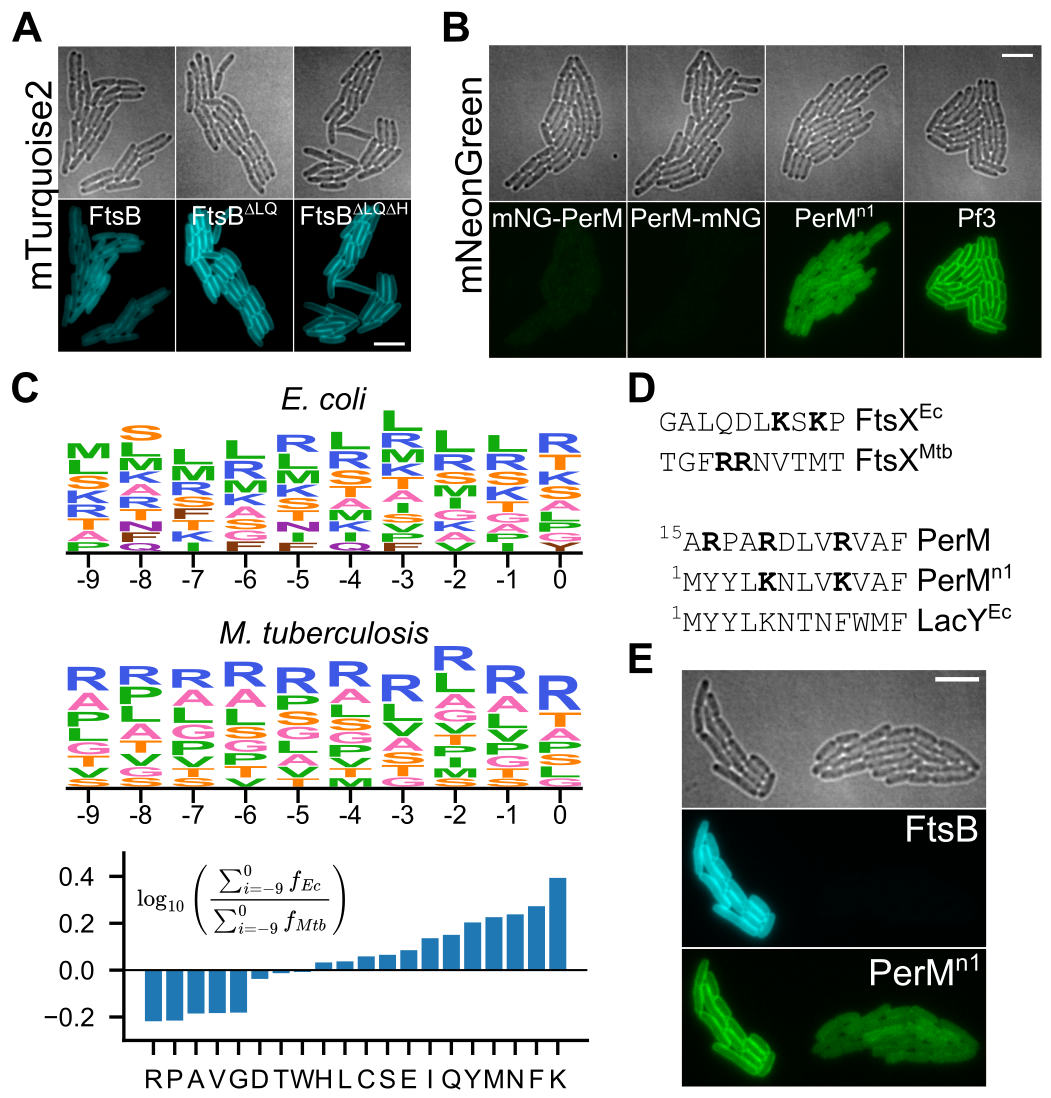
\includegraphics[width=0.5\textwidth]{../figures/fig2.png}
    \caption{
        \textbf{Expression of \mtb{} FtsB and PerM in \ec{}.}
        (\textbf{A}) Expression and membrane localization of FtsB and variants with deletions of \ftsbLQ{} or with deletion of both \ftsbLQ{} and \ftsbH{}. Identical minimum and maximum intensities for mTurquoise2 images.
        (\textbf{B}) Expression and membrane localization for mNG-PerM, PerM-mNG, \permN{}-mNG, and Pf3-mNG. Identical minimum and maximum intensities for mNeonGreen images.
        (\textbf{C}) Top: residue frequency for positions preceding the first predicted transmembrane helix, inclusive of residues found at frequencies above \qty{5}{\percent}. Letter height is proportional to residue frequency with more frequent residues on top. Bottom: relative frequencies in \ec{} and \mtb{}.
        (\textbf{D}) Top: residues preceding the first transmembrane helix in paralogs of FtsX, highlighting lysine and arginine residues. Bottom: comparison of PerM to \permN{} and \ec{} LacY.
        (\textbf{E}) Two adjacent microcolonies from a strain with co-expression of mTq2-FtsB and \permN{}-mNG. The microcolony on the right has coincidentally lost the plasmid encoding mTq2-FtsB, and exhibits reduced membrane localization of \permN{}-mNG. Scale bars \qty{5}{\um}.
    }\label{fig2}
\end{figure}

Conversely, initial attempts to construct mNeonGreen-labeled PerM failed for both N- and C-terminal fusion constructs (mNG-PerM and PerM-mNG; Fig.~\ref{fig2}B).
We manually inspected the predicted PerM structure as well as sequences of integral transmembrane protein orthologs in \ec{} and \mtb{}, hypothesizing that an engineered construct, \permN{}, would exhibit higher expression.
Specifically, we noticed an apparent ``LK'' motif in \ec{} that rarely appeared in \mtb{} and was reminiscent of part of the twin-arginine translocation motif \citep{leeBacterialTwinArginineTranslocation2006}.
Our strategy in designing the \permN{} construct was to modify PerM with aspects of the short LacY N-terminal sequence in ways that would not perturb the predicted PerM structure.
While expression was indeed much higher for \permN{}-mNG, it failed to exhibit the same degree of membrane localization as Pf3-mNG, which we used as a control given its efficient translocation and uniform transmembrane orientation \citep{kieferNegativelyChargedAmino1997}.

We were surprised at how much the modifications in \permN{} increased expression levels and systematically investigated sequences in residues preceding the first predicted transmembrane helix in all proteins including at least one transmembrane helix in the \ec{} and \mtb{} proteomes (Fig.~\ref{fig2}C).
We found large differences in the frequencies of some residues, most strikingly for differences in the relative frequencies of lysine and arginine. Fig.~\ref{fig2}D shows how this is reflected in orthologous sequences of FtsX as well as in \permN{} compared to \mtb{} PerM.
Finally, we proceeded to co-express \permN{}-mNG and mTq2-FtsB and look for evidence of PerM-FtsB interaction.
Serendipitously, one of two adjacent \ec{} microcolonies in a co-expression experiment lost the plasmid for mTq2-FtsB expression (this occasionally happened without including selective antibiotics in agarose gel pads; we note that we used a YFP filter set for mNeonGreen imaging to avoid crosstalk from mTurquoise2).
The large difference in \permN{}-mNG membrane localization between these two microcolonies suggested an unexpected role for FtsB in stabilizing PerM in the \ec{} membrane.

\subsection{PerM stabilization in \ec{} membrane by FtsB depends on \ftsbH{}}

In order to confirm that FtsB increases membrane-localized PerM expression and, if so, to investigate the role of \ftsbH{} in this phenomenon, we co-expressed mNeonGreen- and mTurquoise2-labeled constructs and analyzed fluorescence in \ec{} microcolonies (Fig.~\ref{fig3}).
In these experiments, expression of \permN{}-mNG was induced with \qty{100}{\uM} IPTG. Localization controls mNeonGreen (strong cytoplasmic localization) and Pf3-mNG (strong membrane localization) were induced with \qty{60}{\uM} and \qty{240}{\uM} IPTG, respectively, to match typical \permN{}-mNG expression levels.
Expression of mTurquoise2-labeled FtsB constructs was induced with \qty{10}{\nM} ATc in all conditions except for one condition with no induction (indicated with down arrows in Fig.~\ref{fig3}).
Brightfield images of \ec{} cells were segmented, and protein concentration was estimated to be proportional to total integrated fluorescence after subtracting background and normalizing by cell size.

\begin{figure*}[htb]
\centering
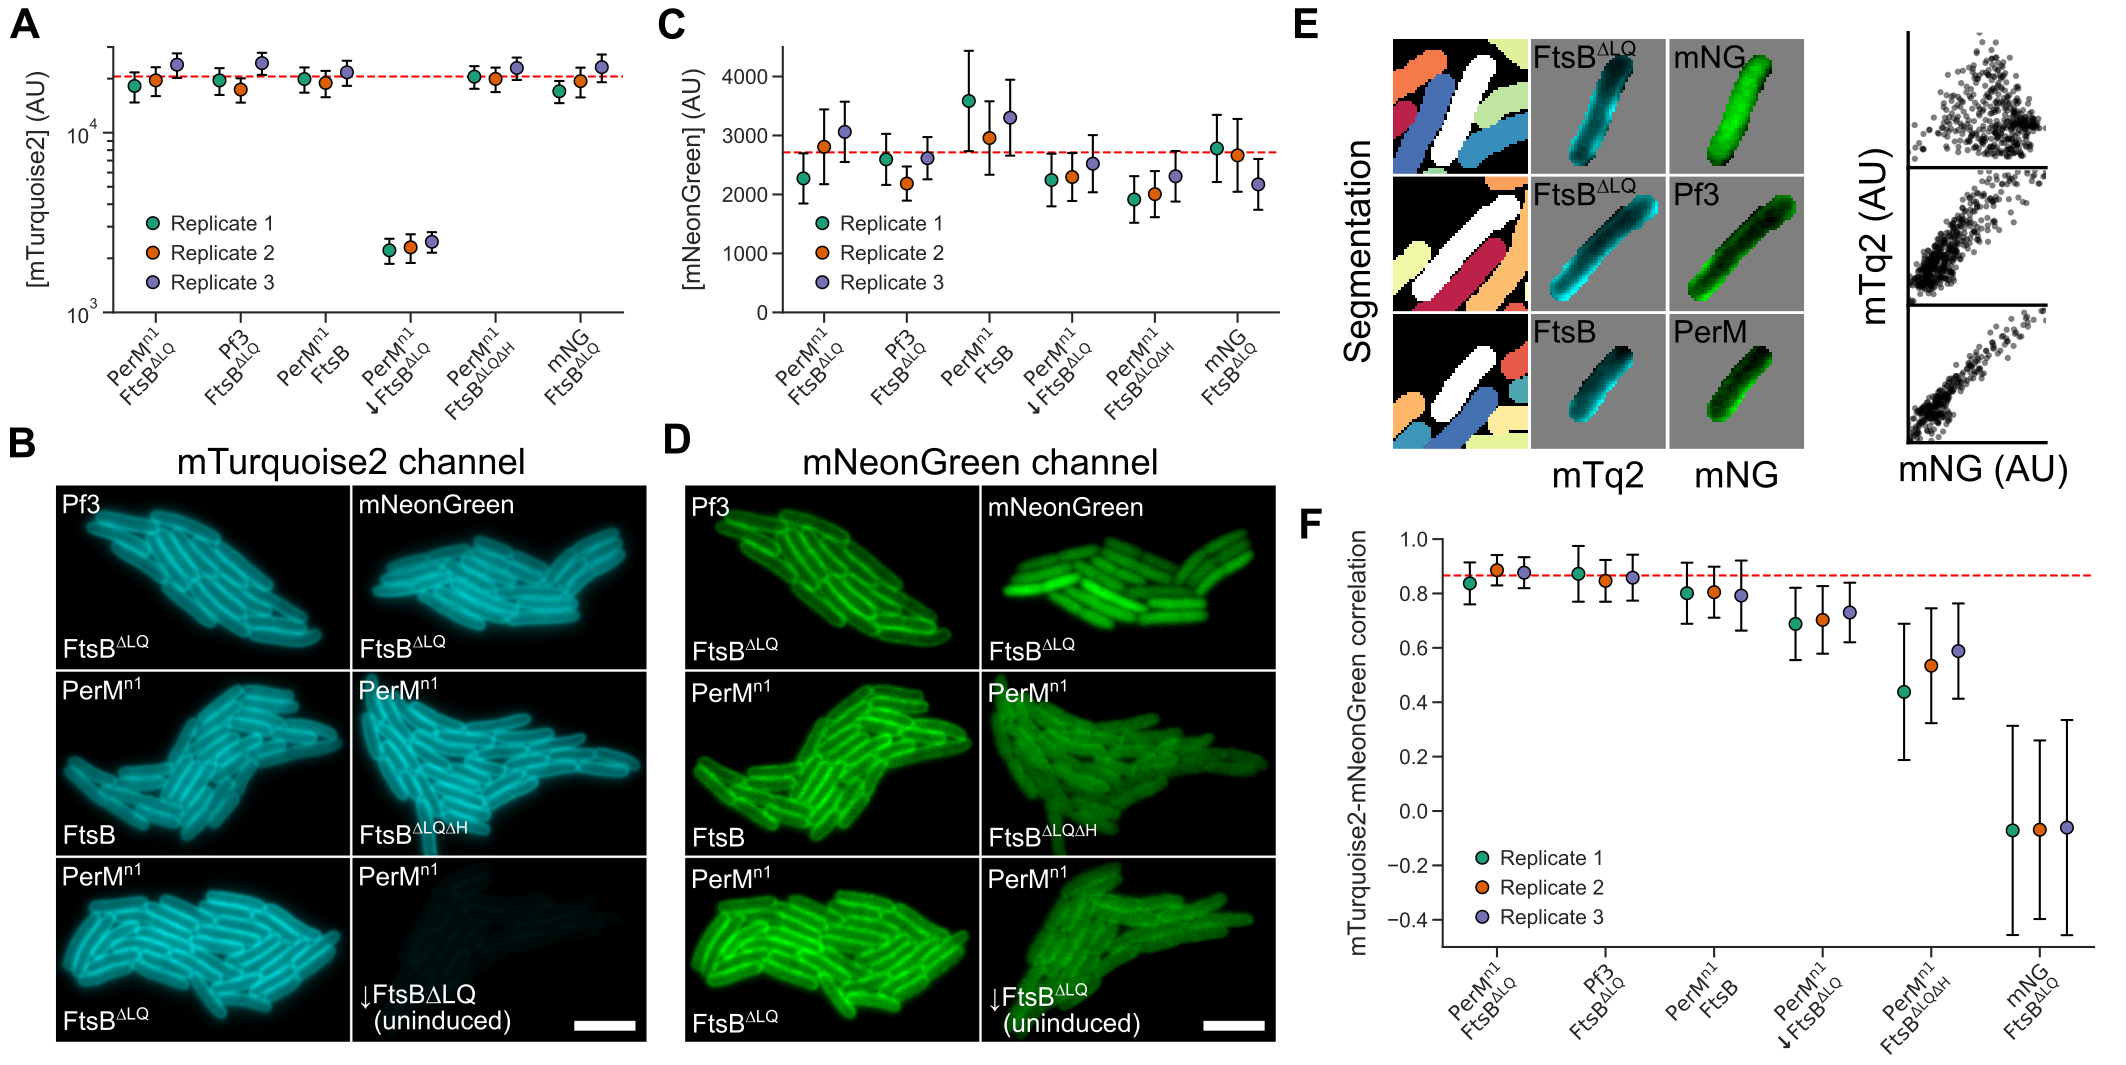
\includegraphics[width=1.0\textwidth]{../figures/fig3.png}
\caption{
    \textbf{FtsB stabilizes PerM in the \ec{} membrane.}
    (\textbf{A}) Distribution of single-cell mTurquoise2 concentration (mean $\pm$ standard deviation) for FtsB constructs in different conditions, each with replicates. Dashed red line indicates the mean value for the reference condition (\permN{}-mNG, mTq2-\ftsbdLQ{}, \qty{100}{\uM} IPTG, \qty{10}{\nM} ATc). Uninduced \ftsbdLQ{} is indicated with a down arrow. A logarithmic scale is used to allow comparison of high- and low-expression conditions.
    (\textbf{B}) Example data from microcolonies for each condition. The uninduced \ftsbdLQ{} condition has very low fluorescence in example data because identical minimum and maximum intensities were used. Scale bar \qty{5}{\um}.
    (\textbf{C, D}) Distribution of single-cell mNeonGreen concentrations and example data for Pf3-mNG, mNeonGreen alone, or \permN{}-mNG in different conditions; prepared identically to \textbf{A} and \textbf{B}.
    (\textbf{E}) Left: example data analysis showing cell segmentation and isolated, single-cell intensities. Right: Scatter plots of single-pixel intensities for each cell show clear correlation for Pf3-mNG and PerM-mNG, but not for mNeonGreen alone. (\textbf{F}) Distribution of single-cell Spearman correlation coefficients (mean $\pm$ standard deviation) for three replicates.
}\label{fig3}
\end{figure*}

Relative to the reference condition (\permN{} and \ftsbdLQ{}, \qty{10}{\nM} ATc), there was an \qty{89}{\percent} ($p=\num{3.3e-12}$) decrease in mTq2-\ftsbdLQ{} expression in the absence of induction, with no significant differences observed for other conditions.
The absence of any significant impact on wild-type FtsB expression ($p=0.97$) compared to when FtsB was expressed in the absence of PerM (compare Fig.~\ref{fig3}B to Fig.~\ref{fig2}A) suggests that \permN{} stabilizes FtsB when expressed in \ec{}, as was observed in \mtb{} \citep{wangPersistentMycobacteriumTuberculosis2019}.
There was also no obvious difference in localization of any FtsB variant in any condition tested.

In contrast, there was a significant reduction in \permN{}-mNG expression of \qty{13.3}{\percent} ($p=\num{3.8e-2}$) in the absence of induction of mTq2-\ftsbdLQ{} expression, and a reduction of \qty{23.5}{\percent} ($p=\num{5.5e-4}$) when \ftsbdLQ{} was replaced with \ftsbdLQdH{}.
There was no significant change when \ftsbdLQ{} was replaced with wild-type FtsB ($p=0.29$). This suggested that FtsB increased PerM stability in \ec{}, and that this depended on the presence of \ftsbH{}.
However, inspection of Fig.~\ref{fig3}C suggests that our sample size is overpowered ($N=\num{10930}$ cells in total from 3 replicates; $607 \pm 44$ cells per condition per replicate) given variation between replicates in mNeonGreen expression levels. 

In preliminary experiments, we observed a large decrease in spatial correlation between mTurquoise2 and mNeonGreen fluorescence when \ftsbdLQ{} was depleted or replaced by \ftsbdLQdH{} (Fig.~\ref{fig3}D).
The observation of small reductions in mNG-\permN{} levels despite apparently large impacts of different FtsB constructs on localization suggested that fluorescent mNeonGreen often remained in the cytoplasm following mNG-\permN{} degradation.
We hypothesized that quantifying spatial correlation would be a more sensitive measurement less susceptible to variation in protein expression levels.
Fig.~\ref{fig3}E shows scatter plots of mNeonGreen and mTurquoise2 intensities for pixels in typical cells with cytoplasmic mNeonGreen, membrane-localized Pf3-mNG, and \permN{}-mNG.
We calculated Spearman correlation coefficients from such distributions for segmented cells and Fig.~\ref{fig3}F shows the mean and standard deviation of correlation coefficients for each condition and replicate.

In the reference condition (\permN{}-mNG, mTq2-\ftsbdLQ, \qty{10}{nM} ATc), correlation was high ($\rho = 0.87$, 0.84--0.89 \qty{95}{\percent} confidence interval) and indistinguishable from that when Pf3-mNG was expressed instead ($p = 0.72$).
All other conditions had significant reductions in correlation. Wild-type FtsB was marginally less well correlated ($\rho = 0.80$, 0.77--0.83).
The apparent reductions in \permN{}-mNG expression levels discussed above were more strongly supported by analysis of spatial correlation, with a drop in correlation in the absence of mTq2-\ftsbdLQ{} induction ($\rho = 0.71$, 0.69--0.73) and a larger drop when mTq2-\ftsbdLQ was replaced with mTq2-\ftsbdLQdH ($\rho = 0.52$, 0.46--0.58).
While \ftsbLQ{} was not absolutely essential for membrane localization of \permN{}, this was also observed in the absence of any FtsB expression (Fig.~\ref{fig2}B).

\subsection{Single-molecule FtsB tracking reveals \ftsbH{}-dependent PerM binding}

Our correlation analysis strongly suggested that FtsB interaction with PerM via \ftsbH{} is key for expression of \permN{} in the membrane.
Since we observed this for transgenic expression in \ec{}, it is unlikely that PerM-FtsB interaction is mediated by host proteins.
However, transient PerM-FtsB interaction could be sufficient for PerM stability without a large fraction of molecules being bound at any time.
If PerM is a significant component in the core \mtb{} divisome as suggested by structure prediction, depletion phenotypes, and midcell localization \citep{goodsmithDisruptionTuberculosisMembrane2015, wangPersistentMycobacteriumTuberculosis2019}, we hypothesized that this implied long-lived PerM-FtsB interactions that could be detected by single-molecule tracking of FtsB diffusion.
FtsB has a single transmembrane helix, while PerM is predicted to have 8 (Fig.~\ref{fig1_1}A); based on the dependence of diffusion of integral membrane proteins on the number of transmembrane helices, we expected a reduction in the FtsB diffusion coefficient from approximately 0.7 to \qty{0.3}{\square\um\per\s} upon PerM binding \citep{lucenaMicrodomainFormationGeneral2018}.

\begin{figure*}[htb]
    \centering
    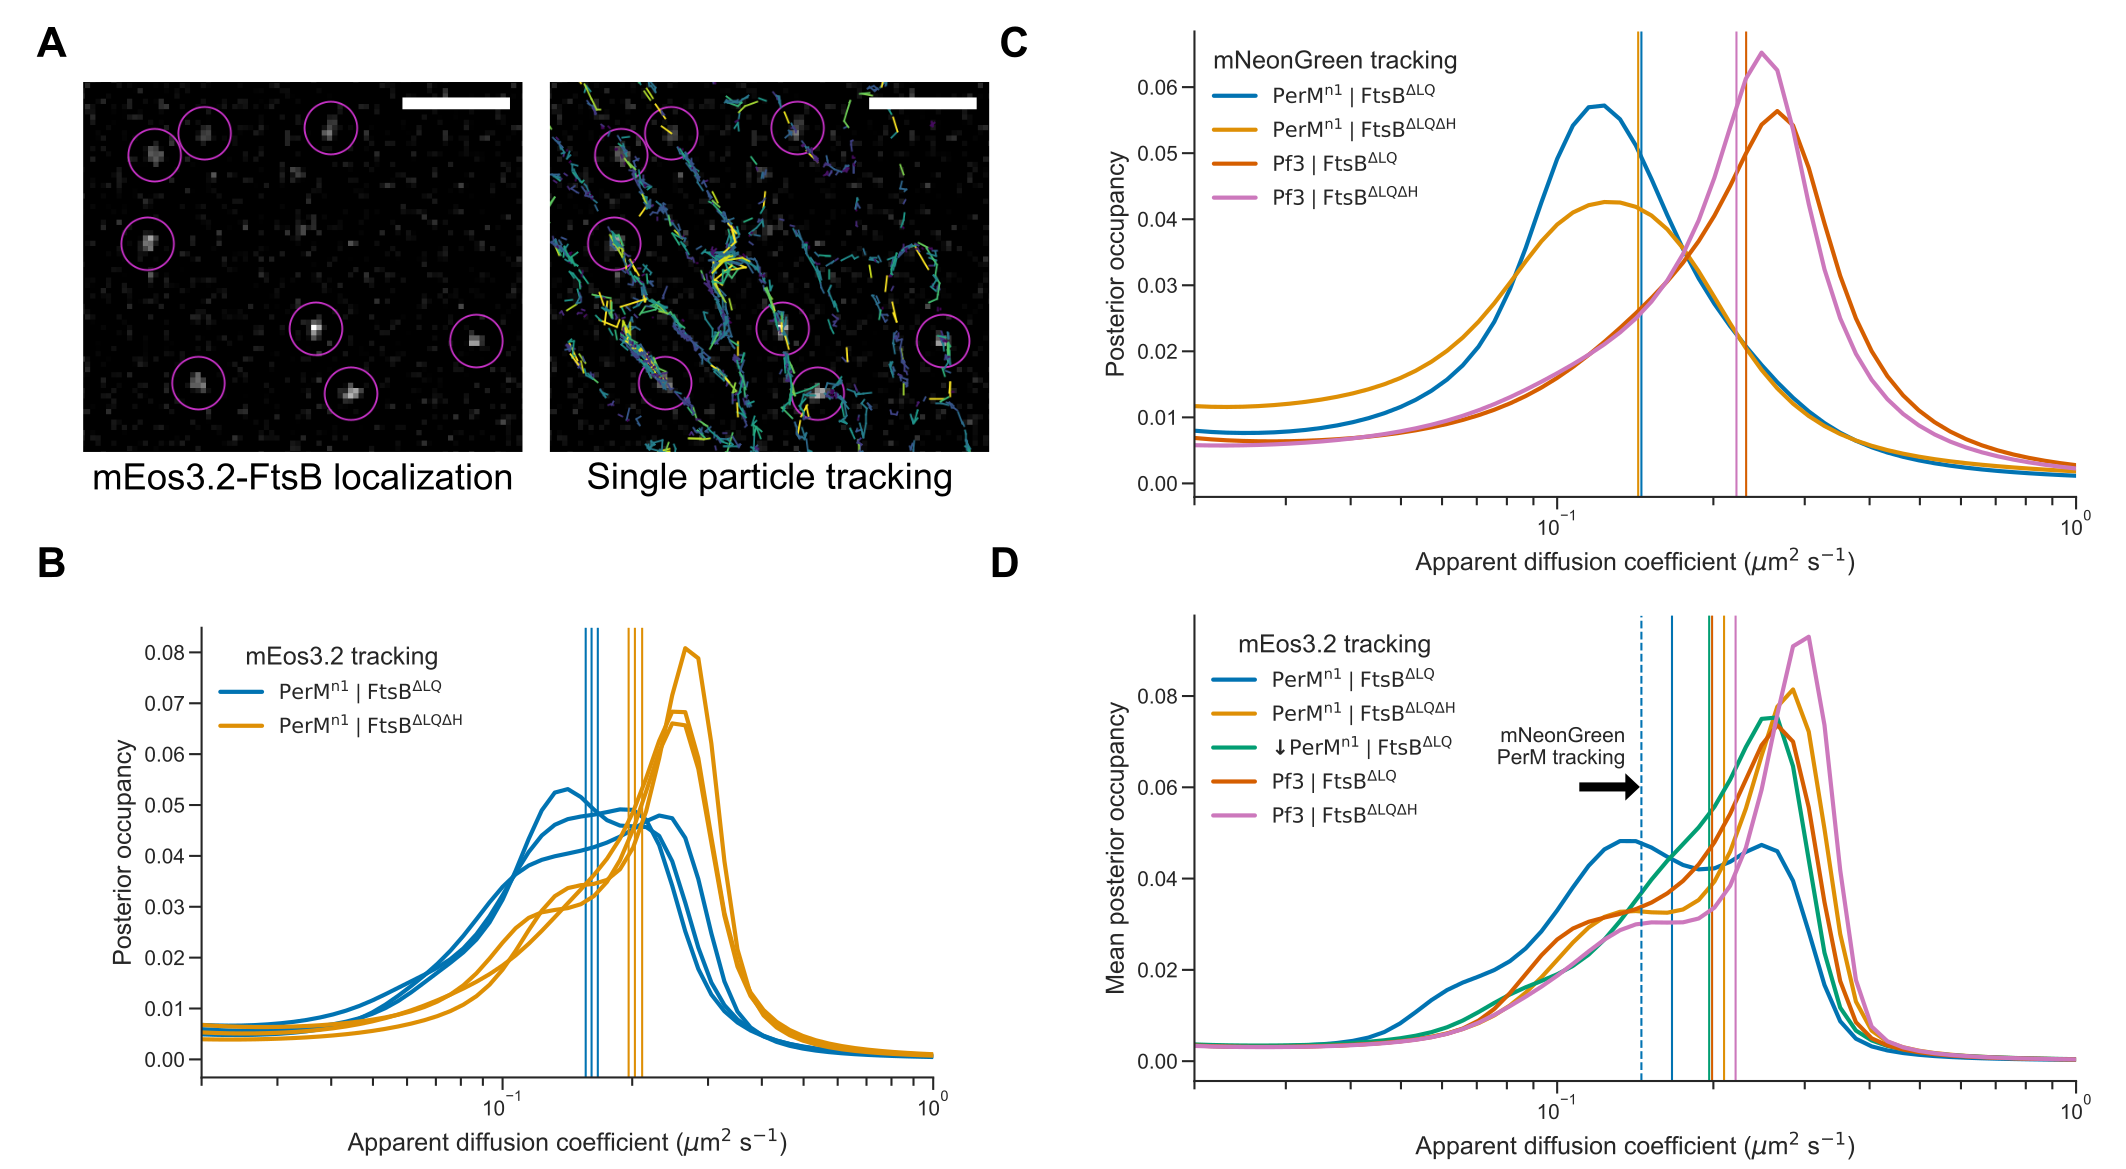
\includegraphics[width=1.0\textwidth]{../figures/fig4.png}
    \caption{
        \textbf{PerM-FtsB binding detected by FtsB single-molecule tracking.}
        (\textbf{A}) Left: single, 33-ms frame from a fluorescence microscopy movie of mEos3.2-\ftsbdLQ{} diffusion in \ec{}. Right: Single-molecule localization and tracking results for the entire movie show membrane-localized diffusion. Scale bar $2~\mu$m.
        (\textbf{B}) Posterior occupancies in a model of regular Brownian motion and localization error were marginalized over localization error to estimate the distribution of apparent 2D diffusion coefficients. Distributions and their means (vertical lines) are shown for three replicates of experiments combining \permN{}-mNG with either mEos3.2-\ftsbdLQ{} or mEos3.2-\ftsbdLQdH{}.
        (\textbf{C}) Estimated distributions of diffusion coefficients inferred from single-molecule tracking of either \permN{}-mNG or Pf3-mNG with either \ftsbdLQ{} or \ftsbdLQdH{} (single experiment). Vertical lines indicate the mean estimated diffusion coefficient for each condition.
        (\textbf{D}) Estimated distribution of diffusion coefficients for either mEos3.2-\ftsbdLQ{} or mEos3.2-\ftsbdLQdH{} co-expressed with either Pf3-mNG or \permN{}-mNG (with or without addition of 100~$\mu$M~IPTG), inferred from combining data from three replicates. Vertical lines indicate mean estimated diffusion coefficients and the dashed vertical line is replicated from \textbf{C}.
    }\label{fig4}
\end{figure*}

We constructed mEos3.2-tagged variants of \ftsbdLQ{} and \ftsbdLQdH{}, and co-expressed them with either \permN{}-mNG or Pf3-mNG.
Fig.~\ref{fig4}A shows a typical frame from single-molecule imaging data, localized mEos3.2 molecules, and single-molecule tracks gathered in one movie showing that tracked molecules were detected near the middle plane of \ec{} cells (approximately \qty{0.5}{\um} from the microscope coverslip).
In analysis of preliminary data, we found that analysis of either mean squared displacement or fitting jump-length distributions was sensitive to variable trajectory length.
Thus, we utilized SASPT \citep{heckertRecoveringMixturesFastdiffusing2022a} to infer distributions of \textit{apparent} diffusion coefficients using a method robust against short trajectories, variable localization error, and defocalization \cite{hansenRobustModelbasedAnalysis2018a}.
Note that we refer to an \textit{apparent} diffusion coefficient, as diffusion within our images is largely confined to the one-dimensional perimeter at the middle plane and, further, confined at the cell poles.
So, while this is sufficient to compare relative diffusion rates in different conditions, precise estimates of diffusion coefficients will require more sophisticated methods and would benefit from 3D tracking over the entire membrane.

In tracking experiments, mEos3.2-FtsB constructs were expressed without induction so that PerM would be in excess and maximize potential binding.
We inferred distributions of diffusion coefficients after marginalizing out localization error for three independent replicates (Fig.~\ref{fig4}B).
We observed reproducible differences in mean diffusion coefficients between \ftsbdLQ{} (\qty{0.161 +- 0.004}{\square\um\per\s}; mean $\pm$ standard deviation) and \ftsbdLQdH{} (\qty{0.203 +- 0.006}{\square\um\per\s}; mean $\pm$ standard deviation).
% PerMn1 FtsBΔLQ mEos3.2 0.1611 0.0043
% PerMn1 FtsBΔLQΔH mEos3.2 0.2033 0.0060
Distributions for both \ftsbdLQ{} and \ftsbdLQdH{} suggested the presence of a slow-diffusion population at approximately \qty{0.14}{\square\um\per\s} that is more prominent for \ftsbdLQ{}.
We also collected single-molecule tracking data for mNG-\permN{} and mNG-Pf3 in single experiments.
Despite limitations of this data (fewer localizations and variable spot density as mNeonGreen photobleaches over time), we inferred average diffusion coefficients of \qty{0.144}{\square\um\per\s} and \qty{0.226}{\square\um\per\s} for mNG-PerM and mNG-Pf3, respectively (Fig.~\ref{fig4}C).
% PerMn1 FtsBΔLQ mEos3.2	0.1665
% PerMn1 FtsBΔLQ mNeonGreen	0.1453
% PerMn1 FtsBΔLQΔH mEos3.2	0.2097
% PerMn1 FtsBΔLQΔH mNeonGreen	0.1433
% PerMn1 uninduced FtsBΔLQ mEos3.2	0.1963
% Pf3 FtsBΔLQ mEos3.2	0.1989
% Pf3 FtsBΔLQ mNeonGreen	0.2313
% Pf3 FtsBΔLQΔH mEos3.2	0.2207
% Pf3 FtsBΔLQΔH mNeonGreen	0.2216
To estimate the most likely apparent diffusion coefficients, we inferred distributions from all data from each condition (Fig.~\ref{fig4}D).
This confirmed that mEos3.2-\ftsbdLQ{}, when expressed with PerM clearly exhibits slower diffusion than when PerM is replaced with Pf3 or in the absence of \ftsbH{}.
Peaks at approximately 0.14 and \qty{0.25}{\square\um\per\s} are consistent with a substantial decrease in the rate of diffusion upon PerM binding.
Out of all other conditions, mEos3.2-\ftsbdLQ{} in the absence of induction of \permN{}-mNG exhibited the slowest diffusion.
However, the effect size was clearly low and further work is required to determine the concentration dependence of this interaction.

\subsection{PerM-FtsB interaction could restrict conformational flexibility of the \mtb{} divisome}

Our observation that \ftsbH{}-dependent PerM-FtsB interaction was sufficiently long-lived to produce large changes in FtsB diffusion prompted us to explore how this interaction could impact the \mtb{} divisome.
We conducted MD simulations to compare divisome constructs in which FtsB was truncated to FtsB\textsuperscript{205} (removing the uncertain C-terminal residues) or truncated to FtsB\textsuperscript{185} (additionally remove \ftsbH{}).
First, we performed MD for the \mtb{} divisome with PerM and full-length FtsB for \qty{500}{\ns}. FtsB N-terminal residues and other terminal residues of subunits without confident structure predictions were omitted.
A period of initial MD was required since our structure prediction did not have all subunits at ideal relative orientations; this was especially significant for FtsQ since its transmembrane helix is distant from others.
The final conformer after \qty{500}{\ns} was used to build systems with truncation to FtsB\textsuperscript{205} (\ftsbdC{}) and to FtsB\textsuperscript{185} (\ftsbdCdH{}), and each system was simulated for \qty{1}{\us}.
The final conformer for \ftsbdC{} is shown in Fig.~\ref{fig5}A.

\begin{figure*}[htb]
    \centering
    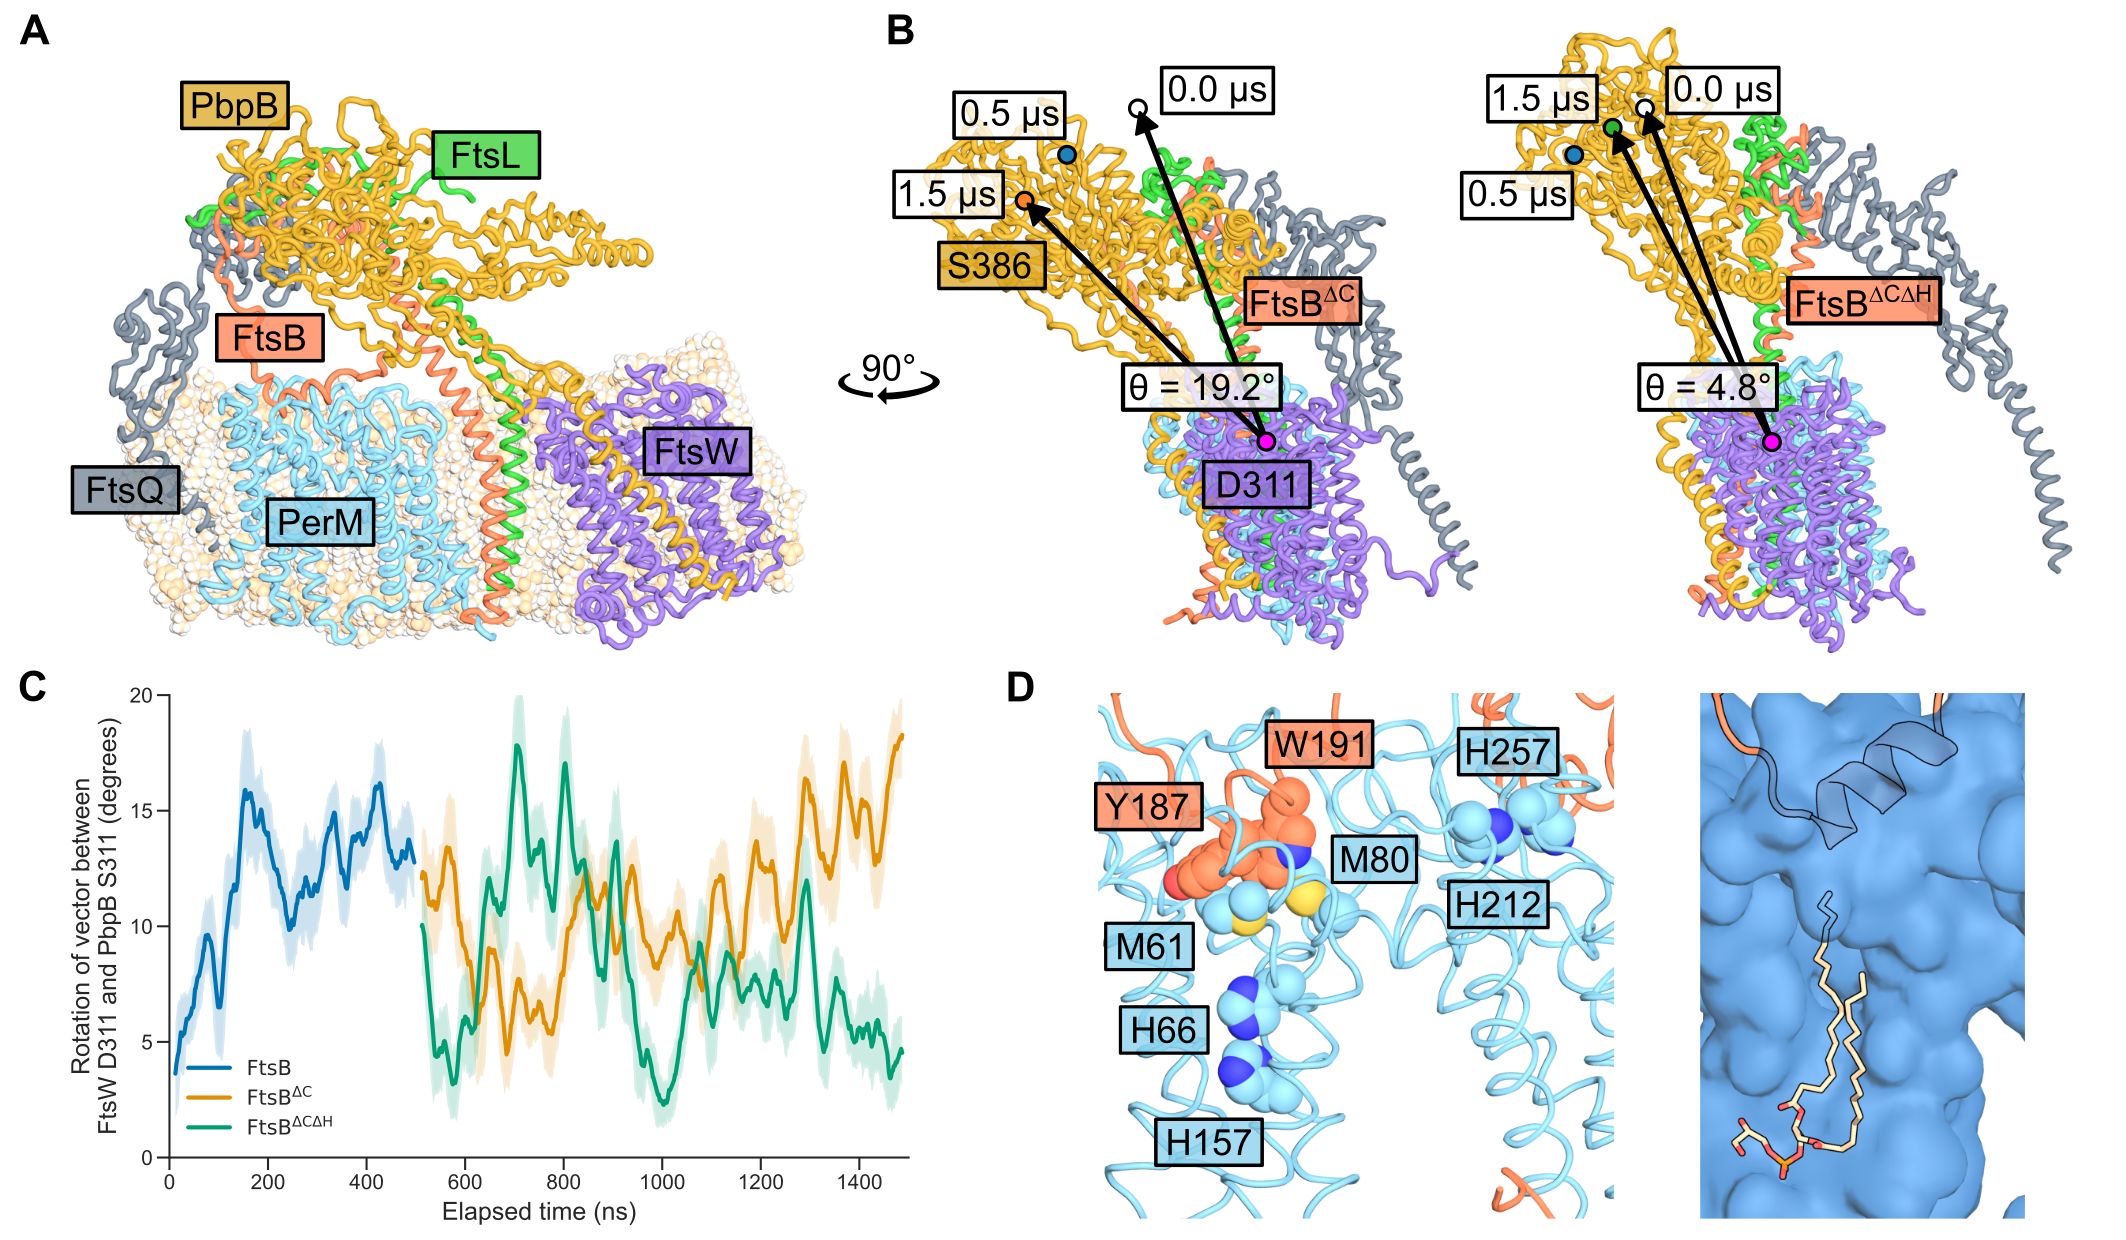
\includegraphics[width=1.0\textwidth]{../figures/fig5.png}
    \caption{
        \textbf{PerM-FtsB interaction constrains the \mtb{} divisome in MD simulations.}
        (\textbf{A}) PerM simulated in context of \mtb{} divisome. Final conformer after \qty{0.5}{\us} of MD with full-length FtsB followed by \qty{1}{\us} of MD with \ftsbdC{}. Note C-terminal truncation of FtsB relative to the predicted structure in \ref{fig1_1} that is uncertain in this region.
        (\textbf{B}) Difference in tilt of PbpB transpeptidase domain relative to its conformation in structure prediction. Final conformers for \ftsbdC{} and \ftsbdCdH{} simulations are shown aligned to FtsW and points show locations of putative active-site residues FtsW\textsuperscript{D311} and PbpB\textsuperscript{S386}. Points at \qty{0}{\us} and \qty{0.5}{\us} are the initial and final positions of PbpB\textsuperscript{S386} in initial simulation using full-length FtsB and are plotted at the same position relative to FtsW.
        (\textbf{C}) Dynamics of tilt angles defined in \textbf{B} show that the \ftsbdCdH{} simulation returned towards the elongated conformation observed in structure predictions. (\textbf{D}) Final conformer of PerM-FtsB after \qty{1.1}{\us} MD. Left: residues in PerM near FtsB-binding interfaces suggest that PerM could potentially be sensitive to environmental cues. Right: a lipid often fills a channel in PerM in MD;  reaching FtsB.
    }\label{fig5}
\end{figure*}

Comparing the final conformers of the \ftsbdC{} and \ftsbdCdH{} simulations, we examined the angle formed as the vector between the putative active site residues FtsW\textsuperscript{D311} and PbpB\textsuperscript{S386} moves during MD simulation (Fig.~\ref{fig5}B).
This angle is a proxy for the tilt of the PbpB transpeptidase domain relative to FtsW that has been used to analyze Cryo-EM data as well as MD simulation.
We observed a \qty{19.2}{\degree} tilt for \ftsbdC{}, similar to that observed for \pa{} FtsI comparing a structure prediction to its Cryo-EM structure \citep{kashammerCryoEMStructureBacterial2023} and for \ec{} comparing a structure prediction to conformers following MD \citep{brittonConformationalChangesEssential2023}.
Conversely, with the loss of PerM-FtsB interaction mediated by \ftsbH{}, the tilt angle reverted to a value within only \qty{4.8}{\degree} of the predicted structure.
The evolution of these angles over the course of MD is shown in Fig.~\ref{fig5}C.

Relative to studies on the divisome in model organisms, there is a paucity of experimental data to relate our simulations to phenotypes associated with mutations to \mtb{} divisome components.
Thus, we did not analyze interactions between \mtb{} divisome subunits in depth or conformations in and around FtsW and PbpB active sites.
However, we note substantial differences the relative conformations of divisome components in final conformers for the \ftsbdC{} and \ftsbdCdH{} simulations; tilt of the PbpB transpeptidase domain was associated with twisting of the PbpB head domain, FtsL, and FtsQ relative to FtsW.
Lastly, in Fig.~\ref{fig5}D we return to the final conformer of a PerM-FtsB simulation following aMD to highlight residues of interest in PerM that are suggestive of potential regulatory mechanisms.
We also show how a phosphatidylglycerol molecule occupies a channel in PerM and interacts with \ftsbH{}.

\section{Discussion}

With our integrative approach combining fluorescence microscopy with molecular dynamics starting from predicted structures of protein complexes, we showed that \ftsbH{} directly mediates PerM-FtsB binding.
Our results are suggestive of significance of PerM-FtsB interaction, going beyond FtsB stabilization \citep{wangPersistentMycobacteriumTuberculosis2019} to potentially impacting the structure of the core \mtb{} divisome.
Given the role of PerM in persistent \mtb{} infection and that it is essential in \msmeg{}, it will be interesting to learn whether FtsB also stabilizes PerM in \mtb{}, as it does in \ec{}, and whether the PerM-FtsB interaction that we have identified can be targeted to disrupt regulation of cell division.

Our approach is straightforward to apply to other predicted protein-protein interactions.
For example, \mtb{} PerM is located in the same operon as Rv0954 which similarly localizes to the \mtb{} divisome yet has no reported deletion phenotype \citep{wangRv0954MemberMycobacterial2021a}.
Intriguingly, while PerM is associated with the divisome component FtsB, Rv0954 exhibited physical and genetic interactions with elongasome components such as RodA and PbpA.
However, division and elongation machinery in mycobacteria are not perfectly analogous to those in other bacteria \cite{baranowskiDreamMycobacterium2019}.
The cell-stress phenotypes of PerM depletion in \mtb{} suggest that conditional phenotypes may be identified for Rv0954 as well.

In Fig.~\ref{fig5}D, we highlight PerM residues that could play roles in integrating environmental stress in proximity to \ftsbH{}.
These include buried histidines that are intriguing with respect to the Mg\textsuperscript{2+}-dependent phenotype of PerM, suggesting sensitivity to nutrient depletion \citep{goodsmithDisruptionTuberculosisMembrane2015}, methionine residues that make hydrophobic interactions with \ftsbH{} and could be sensitive to oxidation, and histidine residues near the membrane surface that could sensitize PerM-FtsB interaction to pH.
Furthermore, in MD we routinely observed lipids to penetrate the first half of PerM and come into contact with FtsB, suggesting the possibility that bilayer composition can directly impact PerM-FtsB interaction.

In our experimental system, transgenic expression of \mtb{} PerM and FtsB in \ec{} makes it likely that we observed effects of direct PerM-FtsB interaction.
This is an advantage of our system as it suggests that PerM-FtsB binding does not depend on phosphorylation or other post-translational modification specific to mycobacteria.
While our single-molecule tracking experiments are not easily extensible to high-throughput investigation, PerM-FtsB and other \mtb{} protein-protein interactions can be explored by adopting our approach to develop FRET interaction reporters based on structures of predicted complexes.
It will also be interesting to see whether our anecdotal success in engineering improved membrane protein expression in \ec{} is applicable to other \mtb{} membrane proteins.

Our approach also carries the inevitable limitations of exploring an interaction in a surrogate system.
It is critical to not extrapolate too much from our experiments before confirming results in \mtb{}.
Our models of the \mtb{} divisome make countless predictions that are testable given the variety of tools for manipulating mycobacterial gene expression and recombineering.
For example, our MD simulations omitted terminal residues in divisome components that are likely functional in some cases.
This is only one example of interactions that we did not predict, but also cannot rule out.
As another example, a specific FtsB-PerM interface was not predicted and did not emerge in MD, but chimeras replacing \ftsbTM{} with an alternative transmembrane helix could determine whether it contributes to PerM binding.

Lastly, our observation that PerM-FtsB interaction constrains PbpB in a tilted conformation can be considered in light of results and discussion emerging from the Cryo-EM structure of the \pa{} divisome \citep{kashammerCryoEMStructureBacterial2023}, where an elongated conformation was considered to potentially reflect the catalytically active state.
Within the context of this model and in light of our results, the role of PerM would be to reduce divisome activity by constraining PbpB in a conformation with relatively low transpeptidase activity. 
This is an apparent paradox given that PerM is essential in some conditions in \mtb{} and in \msmeg{}.
However, the paradox can be resolved if PerM plays both a role in promoting FtsB stability (which can be bypassed with FtsB overexpression \citep{wangPersistentMycobacteriumTuberculosis2019}) and also a conditionally essential role in regulating divisome activity that could contribute to persistent \mtb{} infection.

\section{Methods}

\subsection{Structure prediction}

PerM and FtsB sequences used for structure prediction are listed in Table~\ref{tab1} and additional \mtb{} sequences used for complex structure prediction are listed in Table~\ref{tab2}.
FtsB and PerM were identified in various actinomycete species and, after multiple sequence alignment, have between \qty{19}{\percent} and \qty{61}{\percent} (PerM) and  \qty{27}{\percent} and \qty{62}{\percent} (FtsB) amino acid identity with \mtb{} orthologs.
Protein complex structures were predicted using ColabFold \citep{mirditaColabFoldMakingProtein2022}. Multiple sequences alignments were provided by MMseqs2 \citep{steineggerMMseqs2EnablesSensitive2017} using both paired and unpaired sequences in reference and environmental sequence databases.
AlphaFold-Multimer \citep{evansProteinComplexPrediction2022} (Version 3, Model 4, 12 recycles) was used for structures compared in Fig.~\ref{fig1_1} and Supplementary Fig.~\ref{figS1} and for structure predictions utilized to build MD systems.
PyMOL \citep{delanoPymolOpensourceMolecular2002} was used for all structure visualizations and its \verb|align| function was used to align FtsW structures and to calculate $RMSD$ (using \verb|cycles=0|).

\begin{table*}[htb]
    \caption{GenPept accession numbers for PerM and FtsB sequences used for different actinomycete species.}\label{tab1}%
    % \begin{tabular}{@{}lll@{}}
    \begin{tabularx}{\textwidth}{
        >{\raggedright\arraybackslash}X 
        >{\raggedright\arraybackslash}X 
        >{\raggedright\arraybackslash}X }
    \toprule
    Species                              & PerM accession & FtsB accession \\
    \midrule
    \textit{Mycobacterium tuberculosis}  & NP\_215470     & NP\_215540     \\
    \textit{Mycolicibacterium smegmatis} & WP\_011730590  & WP\_029104417  \\
    \textit{Mycolicibacillus trivialis}  & WP\_085109558  & WP\_085109605  \\
    \textit{Mycolicibacter terrae}       & WP\_085262653  & WP\_085262505  \\
    \textit{Mycobacteroides abscessus}   & WP\_012296377  & WP\_005066469  \\
    \textit{Nocardia asteroides}         & WP\_022566234  & WP\_019049142  \\
    \textit{Gordonia bronchialis}        & WP\_012833219  & WP\_041919790  \\
    \textit{Corynebacterium diphtheriae} & WP\_014318836  & WP\_021334958  \\
    \textit{Actinosynnema pretiosum}     & WP\_157767928  & WP\_253846810  \\
    \textit{Actinopolyspora halophil}    & WP\_026152723  & WP\_017976585  \\
    \botrule
    \end{tabularx}
\end{table*}

\begin{table}[htb]
    \caption{GenPept accession numbers for PerM and FtsB sequences used for different actinomycete species.}\label{tab2}%
    \begin{tabularx}{0.45\textwidth}{
         >{\raggedright\arraybackslash}X 
         >{\raggedright\arraybackslash}X }
    \toprule
    Protein       & Accession  \\
    \midrule
    FtsQ & NP\_216667  \\
    FtsL & NP\_216680  \\
    FtsW & NP\_216670  \\
    PbpB & NP\_216679  \\
    \botrule
    \end{tabularx}
\end{table}

\subsection{Sequence analysis}

To compare PerM and FtsB for different species, multiple sequence alignments were generated using Clustal Omega \citep{sieversFastScalableGeneration2011} and visualized using Biotite \citep{kunzmannBiotiteUnifyingOpen2018}. To compare amino acid frequencies at transmembrane helices, we used DeepTMHMM \citep{hallgrenDeepTMHMMPredictsAlpha2022} to predict the positions of the first transmembrane helix for all proteins in reference proteomes for \ec{} and \mtb{} (UniProt ID UP000000625 and UP000001584). Amino acid frequencies and corresponding sequence logos for the 10 residues preceding the first residue in the first predicted transmembrane helix were calculated and plotted using Logomaker \citep{tareenLogomakerBeautifulSequence2020}.

\subsection{Molecular dynamics}

Molecular dynamics systems were constructed from structures of predicted complexes (or from the final conformer of the initial \qty{500}{\ns} divisome complex simulation) with the CHARMM-GUI Membrane Builder \citep{wuCHARMMGUIMembraneBuilder2014}.
Shared simulation parameters chosen in CHARMM-GUI were: \qty{150}{\mM}~KCl, CHARMM36m forcefield \citep{huangCHARMM36mImprovedForce2017}, \qty{310}{K} temperature, NPT ensemble, and capping all non-native N- and C-terminal residues with ACE and CT3, respectively.
Scripts for OpenMM \cite{eastmanOpenMMRapidDevelopment2017} output by CHARMM-GUI were modified and OpenMM was used for MD simulation. Simulation system sizes are detailed in Table~\ref{tab3}.

\begin{table}[htb]
    \caption{Number of total atoms and numbers and types of lipid residues in MD systems.}\label{tab3}%
    \begin{tabularx}{0.45\textwidth}{llll}
    \toprule
                        & \multicolumn{1}{l}{}            & \multicolumn{2}{c}{Residues}                        \\
    System              & \multicolumn{1}{l}{Atoms} & \multicolumn{1}{l}{POPE} & \multicolumn{1}{l}{POPG} \\
    \midrule
    PerM-FtsB           & 156168                          & 210                      & 70                       \\
    PerM only           & 105155                          & 213                      & 71                       \\
    Complex (FtsB)      & 724208                          & 1246                     & ---                        \\
    Complex (\ftsbdC{})   & 709754                          & 1239                     & ---                        \\
    Complex (\ftsbdCdH{}) & 709645                          & 1239                     & ---           \\
    
    \botrule       
    \end{tabularx}
\end{table}

Simulation systems differed in a few ways (other than small differences in residues included, shown in Table~\ref{tab4}).
First, bilayers simulations for the PerM-FtsB complex and PerM alone included a 3:1 POPE:POPG ratio commonly used for simulations of \ec{} membranes since MD results were compared to \ec{} microscopy data.
Simulations for divisome complexes used pure POPE bilayers, and future work may investigate differences in more complex model membranes \cite{brownMolecularModelingSimulation2023}.
Second, simulations of the PerM-FtsB complex and PerM alone followed a three-stage aMD protocol described in the main text with \qty{2}{\fs} timesteps.
For the aMD stage, OpenMM scripts from CHARMM-GUI \citep{suhCHARMMGUIEnhancedSampler2022} were modified to utilize empirically determined dual boost potentials as previously described for MD of transmembrane proteins \cite{kappelAcceleratedMolecularDynamics2015} and to output a log of applied boost potentials.
We monitored boost potentials applied to dihedral angles and total energy and found the magnitudes of the two boost potentials were similar.
Lastly, divisome complex simulations utilized hydrogen mass repartitioning \citep{gaoCHARMMGUISupportsHydrogen2021} and \qty{4}{\fs} timesteps.

\begin{table*}[htb]
    \caption{Residues included in MD simulation systems.}\label{tab4}%
    \begin{tabularx}{\textwidth}{llXXX}
    \toprule
              &                         & \multicolumn{3}{c}{Divisome systems} \\
    Component & PerM-FtsB and PerM only & FtsB       & \ftsbdC{}    & \ftsbdCdH{}  \\
    \midrule
    PerM      & 11--390                 & 10--385    & 10--385    & 10--385    \\
    FtsB      & 61--204                 & 74--228    & 74--205    & 74--185    \\
    FtsQ      & ---                      & 92--314    & 92--314    & 92--314    \\
    FtsL      & ---                      & 120--232   & 120--232   & 120--232   \\
    FtsW      & ---                      & 41--456    & 41--456    & 41--456    \\
    PbpB      & ---                      & 79--679    & 79--679    & 79--679   \\
    \botrule
    \end{tabularx}
\end{table*}

Atoms of interest for analysis shown in Fig.~\ref{fig1_2}B and Fig.~\ref{fig5}C were identified by investigating sequence alignments to orthologs of FtsB, PbpB, and FtsW to determine conserved \ftsbH{} residues and putative active-site residues.
The MDAnalysis package \cite{gowersMDAnalysisPythonPackage2016, michaud-agrawalMDAnalysisToolkitAnalysis2011} was used to extract trajectories wrapped around the center of mass of protein atoms, to align divisome complex trajectories to FtsW\textsuperscript{60--407} (omitting more mobile cytoplasmic residues), and to extract atomic coordinates.
All-atom coordinates of initial and final conformers as well as protein-only trajectories are available as supplementary data.

\subsection{\ec{} strain construction}

In addition to \mtb{} PerM and FtsB (and variations described in the main text), capsid protein G8P from bacteriophage Pf3 (UniProt identifier P03623; referred to as ``Pf3'' elsewhere in this manuscript) was utilized as a control based upon its small size, efficient translocation, and uniform transmembrane orientation \citep{kieferNegativelyChargedAmino1997}.
Proteins were expressed as translational fusions with fluorescent proteins mTurquoise2 \citep{goedhartStructureguidedEvolutionCyan2012}, mNeonGreen \citep{shanerBrightMonomericGreen2013}, or mEos3.2 \cite{zhangRationalDesignTrue2012}.
No linkers were added between \mtb{} protein sequences and fluorescent proteins as we expected that native termini were disordered based on structure predictions.
Sequences for all proteins were codon-optimized for \ec{} expression.
Plasmids for FtsB-expressing constructs were constructed by isothermal assembly from low-noise, tetracycline-inducible, ampicillin-resistant vectors \citep{henselPlasmidbasedEscherichiaColi2017}.
Plasmids for expression of mNeonGreen as well as mNeonGreen fusions to PerM variants and Pf3 were constructed from IPTG-inducible, spectinomycin-resistant vectors \citep{silvaPlasmidsIndependentlyTunable2019}.
All plasmids and induction conditions used in this study are summarized in Table~\ref{tab5}.

\begin{table*}[htb]
    \caption{\ec{} plasmids utilized in this study and their respective induction conditions. Mutations are described relative to wild-type \mtb{} protein sequences in Table~\ref{tab1} and Table~\ref{tab2}}\label{tab5}%
    \begin{tabularx}{\textwidth}{lllll}
        \toprule
        Plasmid          & Selection     & Induction           & Expressed protein    & Mutation  \\
        \midrule
        pJRF002          & Carbenicillin & \qty{10}{\nM} ATc   & mTq2-FtsB            &  ---  \\
        pJRF007          & Carbenicillin & \qty{10}{\nM} ATc   & mTq2-\ftsbdLQ{}      &  FtsB\textsuperscript{$\Delta$111--163}\\
        pJRF007\_helix  & Carbenicillin & \qty{10}{\nM} ATc   & mTq2-\ftsbdLQdH{}     &  FtsB\textsuperscript{$\Delta$111--163$\Delta$186--194}\\
        pZH904           & Carbenicillin & \qty{10}{\nM} ATc   & mEos3.2-\ftsbdLQ{}   &  FtsB\textsuperscript{$\Delta$111--163}\\
        pLG906           & Carbenicillin & \qty{10}{\nM} ATc   & mEos3.2-\ftsbdLQdH{} &  FtsB\textsuperscript{$\Delta$111--163$\Delta$186--194}\\
        pJRF001          & Spectinomycin & \qty{100}{\uM} IPTG & mNG-PerM             &   --- \\
        pJRF004          & Spectinomycin & \qty{100}{\uM} IPTG & PerM-mNG             &   --- \\
        pJRF004\_n1\_cWT & Spectinomycin & \qty{100}{\uM} IPTG & \permN{}-mNG         &  PerM\textsuperscript{$\Delta$1--23}:MYYLKNLVK   \\
        pJRF010          & Spectinomycin & \qty{240}{\uM} IPTG & Pf3-mNG              &  --- \\
        pZH813           & Spectinomycin & \qty{60}{\uM} IPTG  & mNeonGreen           &  ---  \\          
        \botrule
    \end{tabularx}
\end{table*}

Plasmids were transformed into \ec{} strain MG1655 and selected for growth on \qty{50}{\mg\per\L} carbenicillin and/or spectinomcin in LB or SOB media.
For microscopy experiments, cells were grown overnight from LB plates in rich defined medium \citep{neidhardtCultureMediumEnterobacteria1974} with \qty{0.2}{\percent} glucose (ForMedium Neidhardt Basal Salt Mixture, Glucose \qty{20}{\g\per\L}, and Neidhardt Supplement Mixture, Complete), adjusted to pH 7.4 with KOH.
All cell growth and imaging took place at \qty{37}{\degree\C}.
Consistent with our earlier work, our plasmids allowed for independent induction of co-expressed genes \citep{silvaPlasmidsIndependentlyTunable2019}.
In preliminary experiments, we confirmed that mTurquoise2- and mNeonGreen-labeled proteins could be independently induced, that inducing expression did not impact growth at expression levels utilized in this work, and that there was no significant crosstalk between mTurquoise2 (CFP filter set) and mNeonGreen (YFP filter set).

\subsection{Fluorescence microscopy}

All imaging was done on a Leica DMI6000 inverted microscope using illumination from either a Leica EL6000 source or with laser excitation at \qty{514}{\nm} (mNeonGreen tracking) or combined \qty{405}{\nm} and \qty{561}{\nm} laser excitation (mEos3.2 tracking), adjusting \qty{405}{\nm} laser intensity to achieve acceptable densities of photoactivated mEos3.2 molecules.
Data was acquired using a 100$\times$/1.46 a-plan apochromat oil immersion objective with additional 1.6$\times$ magnification, Leica type F immersion oil, and an Evolve 512 EM-CCD camera (Photometrics), giving a \qty{100}{\nm} pixel size and a narrow depth of field.
Fluorescence images were acquired with three different filter sets: Chroma 49001 (mTurquoise2), Semrock LF514-B (mNeonGreen), and Chroma 69901 (mEos3.2).
Images of example data were composed using Fiji \citep{schindelinFijiOpensourcePlatform2012}, with linear scaling and maintenance of minimum and maximum intensity values for all comparable images.

Microscope samples were prepared by sandwiching agarose gel pads (rich, defined media with \qty{2}{\percent} Invitrogen UltraPure agarose) of approximately \qty{100}{\uL} between microscope slides and acid-cleaned \#1.5H coverslips (Marienfeld).
For all experiments, samples were reinoculated from overnight cultures at a 1:1000 dilution in media including IPTG and/or ATc at specified concentrations, grown for \qty{3}{\hour}, added to a gel pad prepared from the same media, and grown for an additional \qty{1.5}{\hour} before acquiring data.
Microscope sample temperature was held at \qty{37}{\degree\C} using a combination of a heated microscope sample chamber and an objective heater.
This protocol was based on empirical observations that cells reached steady state fluorescence and growth in less than \qty{1}{\hour} after sample preparation, and that excessive cell density led to reduced growth and fluorescence after approximately \qty{3}{\hour}.
In preliminary experiments, we also noted that this combination of growth media and agarose exhibited high background with substantial variation between experiments, found that this could be attributed to agitation while melting agarose.
We subsequently minimized agitation while preparing gel pads.

To obtain comparable data for constructs expected to have different translation initiation rates, we conducted preliminary experiments and determined that \qty{60}{\uM} and \qty{240}{\uM} IPTG induction for plasmids expressing mNeonGreen and Pf3-mNG, respectively, were approximately equivalent to \qty{100}{\uM} IPTG for plasmids expressing \permN{}-mNG.
Protein expression was always induced with IPTG and ATc concentrations listed in Table~\ref{tab5} except in the uninduced conditions indicated by down arrows in figures.
To increase reproducibility in fluorescence correlation and single-molecule tracking analysis, we aimed to image the middle plane of \ec{} cells approximately \qty{500}{\um} from the microscope coverslip.
For fluorescence correlation analysis, we obtained images of 20 fields of cells for each condition in each of 3 independent replicates.
For single-molecule tracking analysis, we obtained streaming movies (\qty{33}{\ms} exposure time) of 5 fields of cells for each condition in each of 3 independent replicates (except for mNeonGreen tracking for which we did not replicate the experiment).
Replicates were obtained on separate days, and sample preparation steps were staggered in time to minimize differences in how samples were handled for each condition.

\subsection{Fluorescence correlation analysis}

Brightfield images were segmented using Omnipose \citep{cutlerOmniposeHighprecisionMorphologyindependent2022}.
The low and variable contrast in our brightfield data produced variation in widths of segmented objects, so objects were morphologically thinned to single-pixel width and then thickened to a uniform width that was more consistent with observed cell morphology.
Sub-pixel channel alignment was achieved by maximizing pairwise cross-correlation of low-pass filtered fluorescence images with inverted brightfield images (\textit{i.e.} mTurquoise2 and mNeonGreen images were aligned to brightfield images---not to each other).
Background intensity was estimated as the mode of a histogram of low-intensity pixels outside of \ec{} cells; in all conditions including uninduced mTq2-\ftsbdLQ{}, cellular autofluorescence was very low relative to signal from fluorescent proteins.
Fluorescence intensities in pixels corresponding to segmented cells after alignment and background subtracted were compared as described in the main text.

For mNeonGreen and mTurquoise2 concentration and correlation comparisons, a mixed linear model was fit to data points from single cells with random slopes and intercepts to allow for day-to-day variation.
Two-tailed p-values were calculated for comparison to the reference condition (\permN{} and \ftsbdLQ{}, \qty{100}{\nM}~ATc) and adjusted for multiple comparisons using the Holm-Šidák method.
Effect sizes are reported for significant results only (adjusted $p<0.05$).
Unless stated otherwise, errors in the manuscript are 1 standard error of the mean.
We followed our designed analysis protocol and manually screened data to identify and exclude image fields that could contribute to outliers (large shifts in sample position, poor focus, or unusual levels of expression for one or both proteins in a microcolony; 32 of 360 in total) and also excluded cells falling outside the middle 95th percentile in either fluorescence intensity or cell area.
However, we found that removing all data filtering steps did not significantly impact differences we observed between experimental conditions.

\subsection{Inference of diffusion coefficient distributions}

We extracted single-molecule trajectories from image stacks using TrackMate \citep{tinevezTrackMateOpenExtensible2017}. Spots were detected using \verb|DogDetector| (\qty{250}{\nm} spot radius) and tracked using \verb|SimpleSpareseLAPTracker| (\qty{500}{\nm} maximum linking distance).
Thresholds were determined empirically for mEos3.2 (160) and mNeonGreen (200) data, and the first 250 frames of mNeonGreen movies were omitted to exclude data before sufficient photobleaching had occurred to acquire single-molecule tracks of mNeonGreen molecules.
Trajectories were \num{3.56 +- 0.03} and \num{3.65 +- 0.11} frames long for mEos3.2 and mNeonGreen, respectively (mean and standard error of the means for 15 mEos3.2 and 4 mNeonGreen experiments).
We then used SASPT \citep{heckertRecoveringMixturesFastdiffusing2022a} to infer posterior distributions of track diffusion coefficients and localization errors, marginalizing out localization distributions for analysis related to Fig.~\ref{fig4}.
Posterior distributions were inferred for log-spaced diffusion coefficients between \num{0.01} and \qty{10}{\square\um\per\s}.
Distributions were normalized to occupancies between \num{0.02} and \qty{1}{\square\um\per\s} to exclude states with highly variable occupancy at the extremes of the diffusion coefficient range.

Our primary analysis used default SASPT parameters (200 iterations of refining state occupancy, trajectories longer than 10 frames split into trajectories 10 frames long or less) and we increased the \verb|sample_size| parameter to avoid subsampling data.
Based on our observation that single-molecule tracks clearly show the perimeter of \ec{} cells at the middle plane, we used \qty{500}{\nm} for the \verb|focal_depth| parameter.
We also note that we manually inspected maximum projections of all image stacks to verify that cells were well focused.
To check for sensitivity to SASPT analysis parameters, we repeated posterior occupancy inference with various conditions: (1) excluding trajectories that were relatively long ($>10$ frames which can arise from fluorescent objects that do not photobleach) or short (2-frame trajectories that can arise from false positive localizations), (2) fixing localization error to \qty{25}{\nm}, and (3) increasing state array refinement to \num{1000} iterations.
We found that SASPT results were robust against parameter choices and that the largest difference was somewhat narrower distribution peaks with increased iterations.

\backmatter

\bmhead{Acknowledgements}

ZH is supported by Fundação para a Ciência e a Tecnologia (FCT) through MOSTMICRO-ITQB (DOI 10.54499/UIDB/04612/2020; DOI 10.54499/UIDP/04612/2020) and LS4FUTURE Associated Laboratory (DOI 10.54499/LA/P/0087/2020).
ZH and RX are supported by a MOSTMICRO-ITQB Exploratory Projects grant.
ZH and JRF thank Sara F. Costa for assistance and insight on this project.
ZH thanks Luísa Guerreiro and Margarida Pereira who worked on this project during internships in our lab.

\bmhead{Data availability}

Plasmids described in this manuscript will be made available through AddGene.
Data and analysis notebooks are available at \url{https://github.com/smmlab/mtb-perm-ftsb}.
Raw microscopy data and MD trajectories (protein atoms only) are available at \url{https://ZENODOURLHERE}.

\bmhead{Author contributions}

JF: molecular cloning, data acquisition, preliminary data analysis and interpretation. RX: data acquisition, data analysis. ZH: structure predictions and simulation, data acquisition, data analysis. All authors wrote and edited the manuscript.

\bibliography{perm-ftsb}% common bib file

\onecolumn
\begin{appendices}

\section{Supplementary Figures}

\begin{figure*}[htb]
\centering
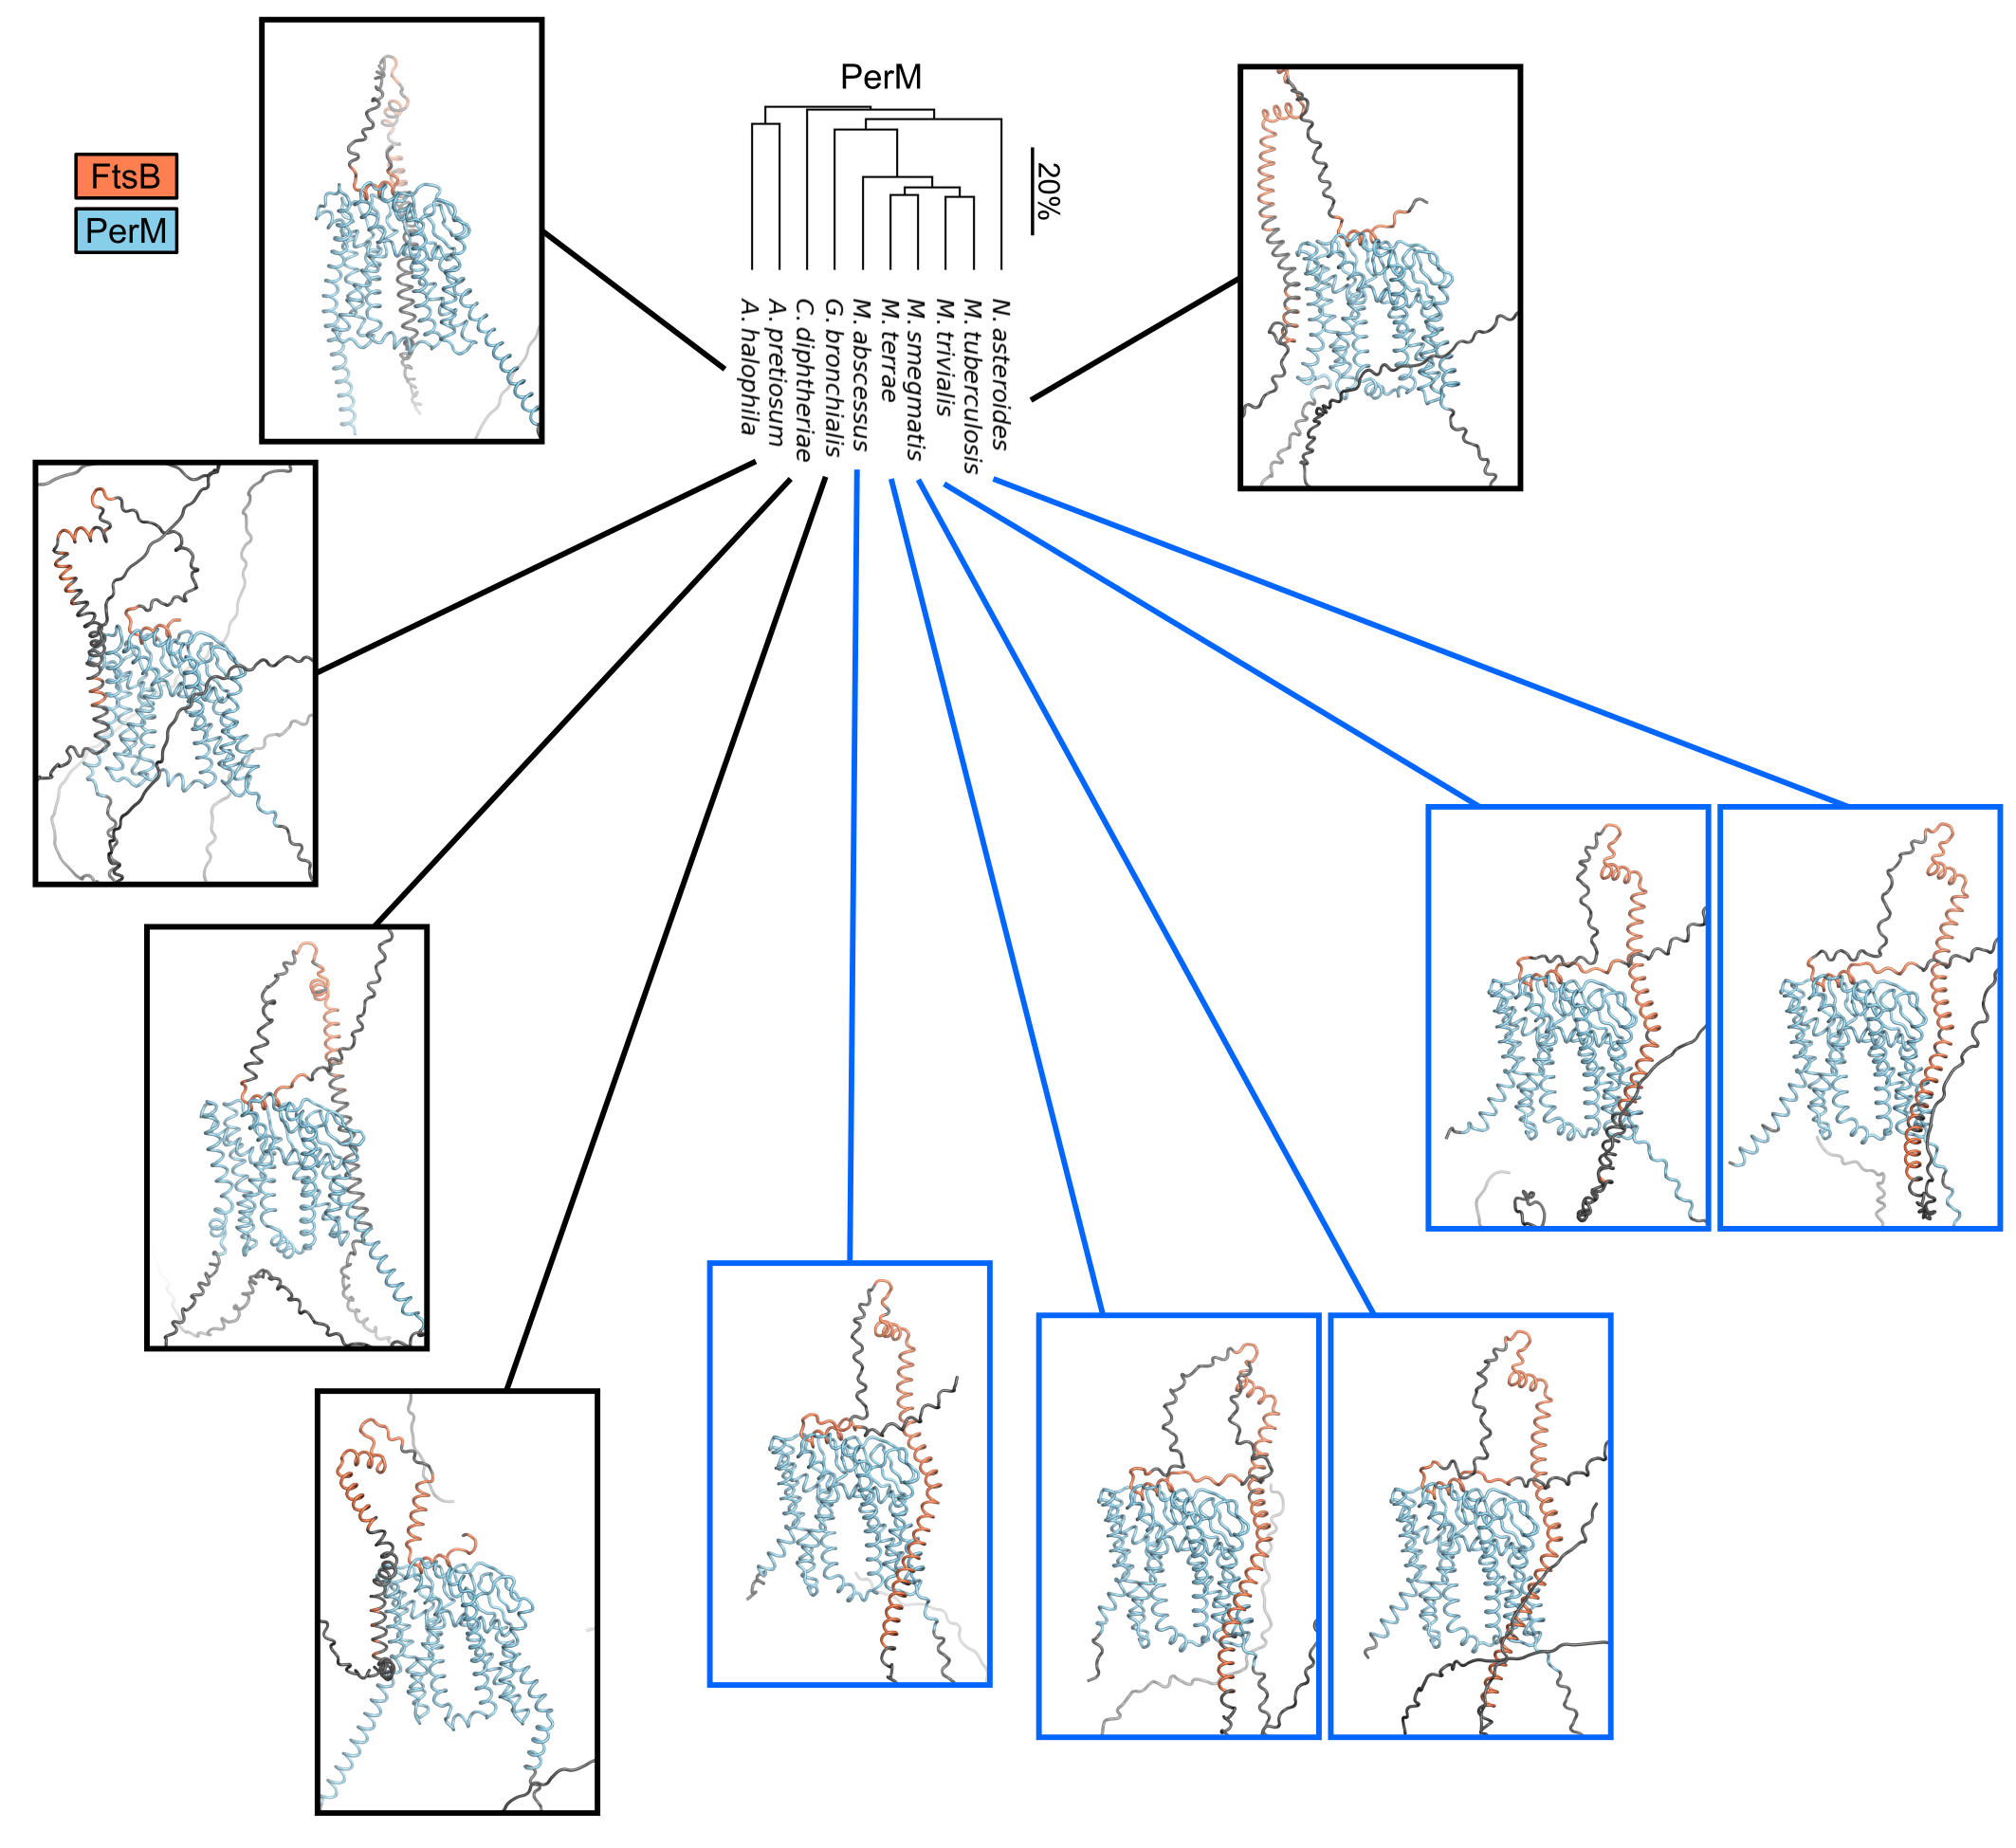
\includegraphics[width=1.0\textwidth]{../figures/figS1.png}
\caption{The PerM phylogenetic tree from Fig.~\ref{fig1_1} is reproduced and compared to PerM-FtsB complexes predicted from full-length sequences for the same species. The predicted orientation of \ftsbTM{} relative to PerM observed for \mtb{} is only observed for more closely related species (blue lines). However, \ftsbH{} interaction with PerM is predicted for all species. Residues with $pLDDT<50$ are colored gray.}\label{figS1}
\end{figure*}

\end{appendices}

\end{document}
